\documentclass[journal abbreviation, manuscript]{copernicus}
\usepackage{enumitem}
\setitemize{noitemsep,topsep=0pt,parsep=0pt,partopsep=0pt}
\usepackage{listings}
\usepackage{xcolor}
\usepackage{longtable}
\usepackage{csvsimple}
\usepackage{flafter}
\usepackage{multicol}
\usepackage[section]{placeins}
\definecolor{codegreen}{rgb}{0,0.6,0}
\definecolor{codegray}{rgb}{0.5,0.5,0.5}
\definecolor{codepurple}{rgb}{0.58,0,0.82}
\definecolor{backcolour}{rgb}{0.95,0.95,0.92}
\usepackage{datatool}
\usepackage{fp}
\let\unit=\unitOld
\usepackage{siunitx}
\usepackage{hyperref}
\usepackage{url}
\hypersetup{
  pdftex,
  colorlinks=true,
  allcolors=blue,
}
\usepackage{hypcap}
\lstdefinestyle{mystyle}{
    backgroundcolor=\color{backcolour},   
    commentstyle=\color{codegreen},
    keywordstyle=\color{magenta},
    numberstyle=\tiny\color{codegray},
    stringstyle=\color{codepurple},
    basicstyle=\ttfamily\footnotesize,
    breakatwhitespace=false,         
    breaklines=true,                 
    captionpos=b,                    
    keepspaces=true,                 
    numbers=left,                    
    numbersep=5pt,                  
    showspaces=false,                
    showstringspaces=false,
    showtabs=false,                  
    tabsize=2
}

\lstset{style=mystyle}
\lstloadlanguages{ 
 Python
}
\begin{document}

\title{The SUMup collaborative database:
Surface mass balance, subsurface temperature and density measurements from the Greenland and Antarctic ice sheets}

\Author[1]{Baptiste }{Vandecrux}
\Author[2]{Charles}{Amory}
\Author[1]{Andreas P.}{Ahlstrøm}
\Author[3]{Pete D.}{Akers}
\Author[4]{Mary}{Albert}
\Author[5]{Richard B.}{Alley}
\Author[2]{Laurent}{Arnaud}
\Author[6]{Ian}{Baker}
\Author[7]{Roger}{Bales}
\Author[8]{Carl}{Benson}
\Author[1]{Jason E.}{Box}
\Author[9]{Christo}{Buizert}
\Author[10, 11]{David M.}{Chandler}
\Author[1]{Charalampos}{Charalampidis}
\Author[12, 13]{Clément}{Cherblanc}
\Author[14]{Nicole}{Clerx}
\Author[1]{William}{Colgan}
\Author[15]{Federico}{Covi}
\Author[16]{Marissa}{Dattler}
\Author[17]{Gilles}{Denis}
\Author[18]{Chris}{Derksen}
\Author[19]{Jack E.}{Dibb}
\Author[20]{Minghu}{Ding}
\Author[21, 22]{Olaf}{Eisen}
\Author[1]{Dominik}{Fahrner}
\Author[1]{Robert}{Fausto}
\Author[2]{Vincent}{Favier}
\Author[23]{Francisco}{Fernandoy}
\Author[21]{Johannes}{Freitag}
\Author[24, 21]{Sebastian}{Gerland}
\Author[25]{Joel}{Harper}
\Author[26]{Robert L.}{Hawley}
\Author[1]{Jasper}{Heuer}
\Author[27]{Regine}{Hock}
\Author[28]{Shugui}{Hou}
\Author[1]{Penelope}{How}
\Author[29]{Bryn}{Hubbard}
\Author[30]{Niel}{Humphrey}
\Author[31]{Yoshinori}{Iizuka}
\Author[24]{Elisabeth}{Isaksson}
\Author[32]{Takao}{Kameda}
\Author[1]{Nanna B.}{Karlsson}
\Author[31]{Kaoru}{Kawakami}
\Author[13]{Helle Astrid}{Kjær}
\Author[33]{Karl}{Kreutz}
\Author[34]{Peter}{Kuipers Munneke}
\Author[35]{Gabriel}{Lewis}
\Author[36]{Michael}{MacFerrin}
\Author[14]{Horst}{Machguth}
\Author[37]{Olivier}{Magand}
\Author[38, 39]{Kenneth D.}{Mankoff}
\Author[40]{Joseph R.}{McConnell}
\Author[41]{Brooke}{Medley}
\Author[42]{Heinrich}{Miller}
\Author[43]{Olivia}{Miller}
\Author[44]{Elizabeth}{Morris}
\Author[45]{Ellen}{Mosley-Thompson}
\Author[15]{Robert}{Mulvaney}
\Author[46]{Masashi}{Niwano}
\Author[26]{Erich}{Osterberg}
\Author[47]{Inès}{Otosaka}
\Author[2]{Ghislain}{Picard}
\Author[48, 4]{Chris}{Polashenski}
\Author[34]{Carleen}{Reijmer}
\Author[49]{Asa}{Rennermalm}
\Author[1]{Anja}{Rutishauser}
\Author[50]{Kirk M.}{Scanlan}
\Author[50]{Sebastian B.}{Simonsen}
\Author[34]{Paul, C.J.P.}{Smeets}
\Author[15]{Andrew}{Smith}
\Author[1]{Anne}{Solgaard}
\Author[51]{Matthew}{Spencer}
\Author[52]{Hans Christian}{Steen-Larsen}
\Author[53, 54]{C. Max}{Stevens}
\Author[31]{Shin}{Sugiyama}
\Author[55]{Jonas}{Svensson}
\Author[56]{Marco}{Tedesco}
\Author[57]{Elizabeth. R}{Thomas}
\Author[58]{Megan}{Thompson-Munson}
\Author[59]{Shun}{Tsutaki}
\Author[1]{Dirk}{van As}
\Author[34]{Michiel R.}{Van den Broeke}
\Author[34]{Maurice}{van Tiggelen}
\Author[60]{Yetang}{Wang}
\Author[21, 61]{Frank}{Wilhelms}
\Author[50]{Mai}{Winstrup}
\Author[49]{Jing}{Xiao}
\Author[62]{Cunde}{Xiao}

\affil[1]{Geological Survey of Denmark and Greenland, Copenhagen, Denmark}
\affil[2]{Université Grenoble Alpes, CNRS, Institut des Géosciences de l'Environnement (IGE), UMR 5001, Grenoble, France}
\affil[3]{Discipline of Geography, School of Natural Sciences, Trinity College Dublin, Dublin, Ireland}
\affil[4]{Thayer School of Engineering, Dartmouth, Hanover, NH, USA}
\affil[5]{Department of Geosciences, and Earth and Environmental Systems Institute, Pennsylvania State University, University Park, PA USA}
\affil[6]{Thayer School of Engineering, Dartmouth College, Hanover, NH, USA}
\affil[7]{University of California, Merced, Merced, CA USA}
\affil[8]{Geophysical Institute, University of Alaska Fairbanks, Fairbanks, Alaska, USA}
\affil[9]{College of Earth Ocean and Atmospheric Sciences, Oregon State University, Corvallis, OR, USA}
\affil[10]{NORCE Norwegian Research Centre and Bjerknes Centre for Climate Research, Bergen, Norway}
\affil[11]{Bristol Glaciology Centre, University of Bristol, Bristol, UK}
\affil[12]{Danish Meteorological Institute, Denmark}
\affil[13]{Niels Bohr Institute, University of Copenhagen, Denmark}
\affil[14]{Department of Geosciences, University of Fribourg, Fribourg, Switzerland}
\affil[15]{British Antarctic Survey, Cambridge, UK}
\affil[16]{University of Maryland, College Park/ NASA Goddard Space Flight Center}
\affil[17]{Imaqa Foundation, Brussels, Belgium}
\affil[18]{Climate Research Division, Environment and Climate Change Canada}
\affil[19]{University of New Hampshire, Durham, NH, USA}
\affil[20]{Chinese Academy of Meteorological Sciences, Beijing, China}
\affil[21]{Alfred-Wegener-Institut, Helmholtz-Zentrum für Polar- und Meeresforschung}
\affil[22]{Universität Bremen}
\affil[23]{Universidad Andrés Bello, Viña del Mar, Chile}
\affil[24]{Norwegian Polar Institute, Tromsø, Norway}
\affil[25]{University of Montana}
\affil[26]{Department of Earth Sciences, Dartmouth College, Hanover, NH, USA}
\affil[27]{Department of Geosciences, University of Oslo}
\affil[28]{School of Oceanography, Shanghai Jiao Tong University, Shanghai, China}
\affil[29]{Aberystwyth University, Aberystwyth, UK}
\affil[30]{Department of Geology and Geophysics, University of Wyoming, Laramie, WY, USA}
\affil[31]{Institute of Low Temperature Science, Hokkaido University}
\affil[32]{Snow and Ice Research Laboratory, Kitami Institute of Technology}
\affil[33]{Climate Change Institute, University of Maine, Orono, ME, USA}
\affil[34]{Institute for Marine and Atmospheric research, Utrecht, The Netherlands}
\affil[35]{Center for Western Weather and Water Extremes, Scripps Institution of Oceanography, University of California, San Diego, La Jolla, CA, USA}
\affil[36]{Cooperative Institute for Research in Environmental Sciences (CIRES), University of Colorado Boulder, Boulder, United States}
\affil[37]{Observatoire des Sciences de l'Univers de la Réunion, UR, CNRS, IRD, météo-France, Saint Denis, La Réunion, France}
\affil[38]{NASA Goddard Institute for Space Studies, New York, NY, 10025 USA}
\affil[39]{Autonomic Integra LLC, New York, NY, 10025 USA}
\affil[40]{Division of Hydrologic Sciences, Desert Research Institute, Reno, NV, USA}
\affil[41]{NASA Goddard Space Flight Center, Earth Sciences Division, Greenbelt, MD, USA}
\affil[42]{Alfred Wegener Institut Helmholtz Zentrum für Polar und Meeresforschung, Bremerhaven, Germany}
\affil[43]{University of Utah, Salt Lake City, USA}
\affil[44]{Scott Polar Research Institute, University of Cambridge}
\affil[45]{Byrd Polar and Climate Research Center, Ohio State University, USA}
\affil[46]{Meteorological Research Institute, Japan Meteorological Agency, Tsukuba, Japan}
\affil[47]{Centre for Polar Observation and Modelling, Northumbria University}
\affil[48]{U.S. Army Cold Regions Research and Engineering Laboratory}
\affil[49]{Rutgers, The State University of New Jersey}
\affil[50]{Geodesy and Earth Observation, DTU-Space, Technical University of Denmark, Lyngby, Denmark}
\affil[51]{Lake Superior State University, Sault Ste. Marie, MI, USA}
\affil[52]{Geophysical Institute, University of Bergen and Bjerknes Centre for Climate Research, Bergen, Norway}
\affil[53]{Earth System Science Interdisciplinary Center, University of Maryland, College Park, MD, USA}
\affil[54]{Cryospheric Sciences Laboratory, NASA Goddard Space Flight Center, Greenbelt, MD, USA}
\affil[55]{Finnish Meteorological Institute, Helsinki, Finland}
\affil[56]{Columbia University}
\affil[57]{British Antarctic Survey, Cambridge UK}
\affil[58]{University of Colorado, Boulder, Colorado, USA}
\affil[59]{National Institute of Polar Research, Tokyo, Japan}
\affil[60]{School of Geography and Environment, Shandong Normal University, Jinan 250014, China}
\affil[61]{Georg-August-Universität Göttingen}
\affil[62]{Beijing Normal University, Beijing, China}

\correspondence{B.Vandecrux (bav@geus.dk)}
\runningtitle{The SUMup collaborative dataset}
\runningauthor{Vandecrux et al.}

\firstpage{1}

\maketitle


% Load CSV files with specified keys
\DTLloadrawdb[keys={index,total,added,nr_references,greenland,antarctica}]{density}{tables//density_meta.csv}
\DTLloadrawdb[keys={index,total,added,nr_references}]{smb}{tables//SMB_meta.csv}
\DTLloadrawdb[keys={index,total,added,nr_references}]{temperature}{tables//temperature_meta.csv}

% Fetch and store the total values from each table
\DTLgetvalueforkey{\DensityTotal}{total}{density}{index}{0}
\DTLgetvalueforkey{\SMBTotal}{total}{smb}{index}{0}
\DTLgetvalueforkey{\TemperatureTotal}{total}{temperature}{index}{0}
\DTLgetvalueforkey{\DensityNew}{added}{density}{index}{0}
\DTLgetvalueforkey{\SMBNew}{added}{smb}{index}{0}
\DTLgetvalueforkey{\TemperatureNew}{added}{temperature}{index}{0}

% Calculate the sum using the fp package
\FPeval{\SumOfTotals}{clip(\DensityTotal+\SMBTotal+\TemperatureTotal)}

\pdfbookmark[1]{Abstract}{abstract}
\begin{abstract}
The SUMup database is a compilation of surface mass balance (SMB), subsurface temperature and density measurements from the Greenland and Antarctic ice sheets available at \url{https://www.doi.org/10.18739/A2M61BR5M} (Vandecrux et al., 2024). This 2024 release contains \num[group-separator={\,}]{\SumOfTotals} data points:  \num[group-separator={\,}]{\SMBTotal} SMB measurements, \num[group-separator={\,}]{\DensityTotal} density measurements and \num[group-separator={\,}]{\TemperatureTotal} subsurface temperature measurements. This is respectively \num[group-separator={\,}]{\SMBNew}, \num[group-separator={\,}]{\DensityNew} and \num[group-separator={\,}]{\TemperatureNew} additional observations of SMB, density and temperature compared to the 2023 release. Since 2023, SUMup provides not only snow accumulation on ice sheets, like its predecessors, but all types of SMB measurements, including from ablation areas. Note that the accumulated SMB is given, not accumulation rates. The data files are provided in both CSV and NetCDF format and contain, for each measurement, the following metadata: latitude, longitude, elevation, timestamp, method, reference of the data source and, when applicable, the name of the measurement group it belongs to (core name for SMB, profile name for density, station name for temperature). Data users are asked to cite all the original data sources that are being used. Issues about this release as well as suggestions of datasets to be added in next releases can be done on a \href{https://github.com/SUMup-database/SUMup-data-suggestion/issues}{dedicated user forum}. We also provide \href{https://github.com/SUMup-database/SUMup-example-scripts}{example scripts to use the SUMup 2024 files} as well as \href{https://github.com/SUMup-database/SUMup-2024-compilation-scripts}{the compilation scripts used to build the database}. SUMup is a community effort and help to compile and curate the database is welcome.

\end{abstract}

\pagebreak
\tableofcontents
\pagebreak
% \copyrightstatement{TEXT}


\pdfbookmark[1]{Introduction: The SUMup project}{intro}
\introduction[The SUMup project]
\pdfbookmark[2]{Background}{bg}
\subsection{Background}
The SUMup database is a community effort to distribute easy-to-use in-situ data to improve surface mass balance modeling and remote sensing efforts, and it is a compilation of work from many individual researchers. It covers measurements of snow and firn density, subsurface temperatures, surface mass balance on the Greenland and Antarctic ice sheets and their peripheral glaciers. After being sponsored by NASA, and by the Scientific Committee on Antarctic Research (SCAR), it is now continued by the Geological Survey of Denmark and Greenland until another group carries it forward. For questions regarding the dataset, please contact the current compiler, Baptiste Vandecrux (bav@geus.dk).


\pdfbookmark[2]{Terms of use}{tou}
\subsection{Terms of use}

When using this dataset, please cite both the individual studies who provided the data (see the reference key given for each measurement and associated reference list) as well as the SUMup dataset itself: 

\bigskip

Vandecrux, B., Amory, C., Ahlstrøm, A.P., Akers, P.D., Albert, M., Alley, R.B., Arnaud, L., Baker, I., Bales, R., Benson, C., Box, J.E., Buizert, C., Chandler, D.M., Charalampidis, C., Cherblanc, C., Clerx, N., Colgan, W., Covi, F., Dattler, M., Denis, G., Derksen, C., Dibb, J.E., Ding, M., Eisen, O., Fahrner, D., Fausto, R., Favier, V., Fernandoy, F., Freitag, J., Gerland, S., Harper, J., Hawley, R.L., Heuer, J., Hock, R., Hou, S., How, P., Hubbard, B., Humphrey, N., Iizuka, Y., Isaksson, E., Kameda, T., Karlsson, N.B., Kawakami, K., Kjær, H.A., Kreutz, K., Kuipers Munneke, P., Lewis, G., MacFerrin, M., Machguth, H., Magand, O., Mankoff, K.D., McConnell, J.R., Medley, B., Miller, H., Miller, O., Morris, E., Mosley-Thompson, E., Mulvaney, R., Niwano, M., Osterberg, E., Otosaka, I., Picard, G., Polashenski, C., Reijmer, C., Rennermalm, A., Rutishauser, A., Scanlan, K.M., Simonsen, S.B., Smeets, P.C., Smith, A., Solgaard, A., Spencer, M., Steen-Larsen, H.C., Stevens, C.M., Sugiyama, S., Svensson, J., Tedesco, M., Thomas, E.R., Thompson-Munson, M., Tsutaki, S., van As, D., Van den Broeke, M.R., van Tiggelen, M., Wang, Y., Wilhelms, F., Winstrup, M., Xiao, J., Xiao, C.: The SUMup collaborative database: Surface mass balance, subsurface temperature and density measurements from the Greenland and Antarctic ice sheets (2024 release), Arctic Data Center, \url{https://www.doi.org/10.18739/A2M61BR5M}, 2024.

\pdfbookmark[2]{Contributing to the Dataset}{contrib}
\subsection{Contributing to the Dataset}
If you would like to contribute to the dataset, reach out to Baptiste Vandecrux (bav@geus.dk) for more details.

\pdfbookmark[2]{Acknowledgement}{acknowledgement}
\subsection{Acknowledgement}

The SUMup working group was previously supported by the NASA Cryospheric Sciences Program and the National Science Foundation and the SCAR AntClimNow Dataset Stewardship grant. Now the maintenance of this dataset is supported by the Programme for Monitoring of the Greenland ice sheet (PROMICE), which is supported by the Danish Ministry for Environment, Energy and Utilities.

\bigskip

We are also grateful to all the people that helped collecting these data. We here thank H., Anschütz, J.R., Banta, N., Bertler, H., Conway, D., Divine, D., Dixon, A., Ekaykin, H., Fischer, R., Forster, M., Frezzotti, T., Fudge, S., Fujita, J., Gallet, B., Goodwin, K., Graeter, W., Graf, M., Hastings, A., Heilig, K., Jezek, K., Keegan, T.V., Khodzher, L., Koenig, J.Y., Lindsey-Clark, P., Martinerie, P., Mayewski, H., Oerter, H., Oerter, A., Ohmura, M., Philippe, J.L., Roberts, E., Schlosser, B., Stenni, K., Takahashi, P., Vallelonga, B., Vinther, D., Vladimirova and C., Vos who either declined co-authorship, failed to answer the invitation or whose updated contact detail could not be found. We also thank L. Koenig, J.T.M. Lenaerts, L. Montgomery, C. Miège, P. Zens, L. Lolk Hauge, who continued their career in the private sector and eventually our departed colleagues and pioneers of the field: K. Steffen (2020), D. Wagenbach (2016), H.B. Clausen (2013).

\bigskip

Eventually, the SUMup database could not exist without all the institutions funding research, expeditions and monitoring in Greenland and Antarctica, among which: the Belgian Federal Science Policy Office and its Research Programme on the Antarctic, the Belgian Fund for Scientific Research, Canada's Natural Sciences and Engineering Research Council (NSERC), China's National Key Research and Development Program, the National Natural Science Foundation of China and Chinese Academy of Sciences, Denmark's Independent Research Fund, the Villum, Carlsberg and A. P. Møller Foundations, the University of Copenhagen and the Danish Ministry for Environment, Energy and Utilities, the European Research Council (ERC), the European Space Agency, the French National Centre for Scientific Research and its Glacioclim Observatory, the German Research Foundation and the Helmholtz Association of German Research Centres, Japan's Society for the Promotion of Science, National Institute of Polar Research and Arctic Challenge for Sustainability, and Japan's Ministry of Education, Culture, Sports, Science and Technology (MEXT), the Fondation Albert 2 de Monaco, the Netherland's Institute for Scientific Research, Earth System Science Centre and Royal Academy of Sciences, Norway's University of Bergen and Trond Mohn Foundation, Sweden's national nuclear waste management organisation (SKB) through it Greenland Analog Project (GAP), the Swiss National Science Foundation, UK's Natural Environment Research Council, the U.S. National Science Fundation (NSF), National Aeronautics and Space Administration (NASA), and U.S. army's Cold Regions Research and Engineering Laboratory (CRREL), the Climate Change Consortium of Wales, the international consortiums such as Vostok, EUROCORE, Law Dome TALDICE, GRIP, EastGRIP, NGRIP, GISP, GISP2 as well as all the organisations supporting these expeditions in the field: CH2M HILL Polar Services, Institut polaire français Paul-Émile Victor, International Polar Foundation, UNAVCO, the U.S. Ice Drilling Program, the US Air National Guard, Asiaq Greenland Survey, and many others.


\pdfbookmark[1]{Important notes for the 2024 release}{list}
\section{Important notes for the 2024 release}

\textbf{All SMB observations are given as cumulative values in meters water equivalent}. Users therefore need to always use the \texttt{SMB} value in combination with the \texttt{start\_year} and \texttt{end\_year} or \texttt{start\_date} and \texttt{end\_date}. A yearly \texttt{SMB} value given for year \texttt{Y} will be reported with \texttt{start\_year = end\_year = Y} and with \texttt{start\_date = end\_date = NaN}. Subannual \texttt{SMB} values will be reported, for instance, with \texttt{start\_year = end\_year = Y} and \texttt{start\_date = 'YYYY-01-01'}, \texttt{end\_date = 'YYYY-02-01'}.

\bigskip


To preserve all special characters in references and location names, all strings in the netCDF files have been saved as UTF-8 instead of the ASCII format used previously. To ensure that the strings are decoded properly, you can use the following code:

\begin{lstlisting}[language=python]
import xarray as xr
import numpy as np

path_to_sumup = '.'
# loading data
df_sumup = xr.open_dataset(path_to_sumup+'/SUMup_2024_SMB_greenland.nc',
                           group='DATA')
# loading metadata
ds_meta = xr.open_dataset(path_to_sumup+'/SUMup_2024_SMB_greenland.nc',
                           group='METADATA')

# small function to decode the string
decode_utf8 = np.vectorize(lambda x: x.decode('utf-8') if isinstance(x, bytes) else x)
# applying this function to all variables that have string as type
for v in ['name','reference','reference_short','method']:
    ds_meta[v] = xr.DataArray(decode_utf8(ds_meta[v].values), dims=ds_meta[v].dims)
\end{lstlisting}

See example scripts to use the SUMup files here: \url{https://github.com/SUMup-database/SUMup-example-scripts}



\pdfbookmark[1]{List of datasets added to the 2024 release}{list}
\section{List of datasets added to the 2024 release}
\pdfbookmark[2]{New surface mass balance data}{newSMB}
\subsection{New surface mass balance data}

Greenland:
\bigskip

\noindent\fbox{%
    \parbox{\textwidth}{%
\begin{multicols}{2}
    \begin{itemize}
    \item Daily ablation data from the Leverett glacier Chandler et al. (2015, 2021)
	\item Daily ablation from at the Historical GC-Net AWS (Steffen et al., 1996, Vandecrux et al., 2023)
    \item Daily ablation from the IMAU AWS (Smeets et al., 2018)
    \item Continuous measurement of SWE from SnowFox instruments (Fausto, 2021)
    \item Accumulation from Operation Ice Bridge radar surveys from Koenig et al. (2016)
    \item Added historical ice cores from Crete and Milcent
    \item Re-added ACT10 radar profiles with original coordinates
    \item Re-added the PARCA cores from Mosley-Thompson et al. (2001) including three datation techniques
    \item Fixed issues inherited from previous releases
    \end{itemize}
\end{multicols}
    }%
}

\bigskip
Antarctica:
\bigskip

\noindent\fbox{%
    \parbox{\textwidth}{%
\begin{multicols}{2}
    \begin{itemize}
    \item Added all data from Ant2k compilation (Thomas et al., 2017)
    \item Added all data from AntSMB compilation (Wang et al., 2021)
    \item Fixed coordinates and references in the compiled data
    \item Added monthly accumulation measurement from stake farm at the Amundsen-Scott South Pole station (South Pole Meteorology Office, 2024)	
    \end{itemize}
\end{multicols}
    }%
}

\subsection{New density data}

Greenland:
\bigskip

\noindent\fbox{%
    \parbox{\textwidth}{%
\begin{multicols}{2}
    \begin{itemize}
    \item GC-Net 2024 field work snow pit and firn cores (Vandecrux et al., 2023)
    \item Harper and Humphrey (2023) cores on EGIG line
    \item Rasmussen et al., (2023) densities at EastGRIP
    \end{itemize}
\end{multicols}
    }%
}

\bigskip
Antarctica:
\bigskip

\noindent\fbox{%
    \parbox{\textwidth}{%
\begin{multicols}{2}
    \begin{itemize}
    \item Sipple Dome 1996-1997 data
    \item RICE core densiies (Winstrup et al., 2019)
    \item Densities compiled by Picard et al., (2022)
    \item South Pole ice core densities from Winski et al. (2019)
    \item GlacioClim-SAMBA densities for traverses between 2004-2024
    \item Brazilian ice cores: Taveres et al. (2020), Marques et al. (2014), Portella et al. (2023), Hammes et al. (2009), Schwanck et al. (2014, 2016), Marcher et al. (2022), Ferreira et al. (2024), Marquetto et al. (2020), Simoes et al. (2004a, 2004b), Gerhard et al. (2018)
    \item Ice cores from Dome C and, D47 and D57 from Verfaillie et al. (2012), Raynaud and Barnola (1985) and Arnaud et al. (1998)
    \item Fixed issues inherited from previous releases
    \end{itemize}
\end{multicols}
    }%
}

\subsection{New temperature data}

Greenland:
\bigskip

\begin{itemize}
\item In 2023, data prepared for Vandecrux et al. (2024) were distributed as monthly averaged, 10 m temperatures. In this new release, all the data collected for Vandecrux et al. (2024) is distributed at all available depths and on daily averages.
\item 2024 data for PROMICE and GC-Net stations (Fausto et al., 2021, How et al., 2022)
\item 2024 data for the deep temperature string at Camp Century (Colgan et al., 2017, Vandecrux et al., 2021)
\item 2023 and 2024 temperature data from Saito et al. (2024); Harper and Humphrey (2023, 2023)
\item Snow temperature data from SIGMA-A station: Nishimura et al. (2023)
\end{itemize}


\bigskip

Antarctica: No temperature addition for 2024.

\section{The density data files}
\subsection{NetCDF files}

All variables are packed in 
\begin{itemize}
\item SUMup\_2024\_density\_antarctica.nc
\item SUMup\_2024\_density\_greenland.nc
\end{itemize}

Due to different dimensionality, the DATA and METADATA variables are saved as two different groups in the NetCDF files

In python:
\begin{lstlisting}[language=python]
import xarray as xr
import numpy as np

path_to_SUMup_folder = "."
ds_density = xr.open_dataset(
    path_to_SUMup_folder + 'SUMup_2024_density_greenland.nc', 
    group='DATA'
    )
ds_meta = xr.open_dataset(
    path_to_SUMup_folder + 'SUMup_2024_density_greenland.nc',
    group='METADATA'
    )
# small function to decode the string
decode_utf8 = np.vectorize(lambda x: x.decode('utf-8') if isinstance(x, bytes) else x)
# applying this function to all variables that have string as type
for v in ['name','reference','reference_short','method']:
    ds_meta[v] = xr.DataArray(decode_utf8(ds_meta[v].values), dims=ds_meta[v].dims)
\end{lstlisting} 


\subsection{CSV files}
The “DATA” variables are given in the following comma-delimited (CSV) files 
\begin{itemize}
\item SUMup\_2024\_density\_antarctica.csv 
\item SUMup\_2024\_density\_greenland.csv 
\end{itemize}

while the “METADATA” variables are given in the tab-delimited (TSV) files
\begin{itemize}
\item SUMup\_2024\_density\_methods.tsv
\item SUMup\_2024\_density\_profile\_names.tsv
\item SUMup\_2024\_density\_references.tsv
\end{itemize}

\begin{table}[t]
\caption{Variables within the density NetCDF file}
\begin{tabular}{|llll|}
\hline
\multicolumn{1}{|l|}{\textbf{Variable}} &
  \multicolumn{1}{l|}{\textbf{Long name}} &
  \multicolumn{1}{l|}{\textbf{Unit}} &
  \textbf{Description} \\ \hline
  
\multicolumn{4}{|l|}{\textbf{DATA VARIABLES}} \\ \hline
\multicolumn{1}{|l|}{measurement\_id} &
  \multicolumn{1}{l|}{measurement\_index} &
  \multicolumn{1}{l|}{-} &
  index of density measurement (unique for each observation) \\ 
\multicolumn{1}{|l|}{timestamp} &
  \multicolumn{1}{l|}{timestamp} &
  \multicolumn{1}{l|}{\begin{tabular}[c]{@{}l@{}}days since \\ 1900-01-01\end{tabular}} &
  date at which measurement \textless{}measurement\_id\textgreater was measured \\ 
\multicolumn{1}{|l|}{start\_depth} &
  \multicolumn{1}{l|}{start\_depth\_of\_measurement} &
  \multicolumn{1}{l|}{m} &
  top depth of density measurement \textless{}measurement\_id\textgreater{} \\ 
\multicolumn{1}{|l|}{stop\_depth} &
  \multicolumn{1}{l|}{stop\_depth\_of\_measurement} &
  \multicolumn{1}{l|}{m} &
  bottom depth of density measurement \textless{}measurement\_id\textgreater{} \\ 
\multicolumn{1}{|l|}{midpoint} &
  \multicolumn{1}{l|}{midpoint\_depth\_of\_measurement} &
  \multicolumn{1}{l|}{m} &
  midpoint depth of density measurement \textless{}measurement\_id\textgreater{} \\ 
\multicolumn{1}{|l|}{density} &
  \multicolumn{1}{l|}{density} &
  \multicolumn{1}{l|}{kg m$^{-3}$} &
  measured density for measurement \textless{}measurement\_id\textgreater{} \\ 
\multicolumn{1}{|l|}{error} &
  \multicolumn{1}{l|}{error} &
  \multicolumn{1}{l|}{kg m$^{-3}$} &
  \begin{tabular}[c]{@{}l@{}}Error associated with the density measurement \\ \textless{}measurement\_id\textgreater{}\end{tabular} \\ 
\multicolumn{1}{|l|}{latitude} &
  \multicolumn{1}{l|}{latitude} &
  \multicolumn{1}{l|}{degree North} &
  latitude of measurement \textless{}measurement\_id\textgreater{} \\ 
\multicolumn{1}{|l|}{longitude} &
  \multicolumn{1}{l|}{longitude} &
  \multicolumn{1}{l|}{degree East} &
  longitude of measurement \textless{}measurement\_id\textgreater{} \\ 
\multicolumn{1}{|l|}{elevation} &
  \multicolumn{1}{l|}{elevation} &
  \multicolumn{1}{l|}{m} &
  elevation of measurement \textless{}measurement\_id\textgreater (datum may vary) \\ 
\multicolumn{1}{|l|}{profile\_key} &
  \multicolumn{1}{l|}{profile\_key} &
  \multicolumn{1}{l|}{-} &
  profile key associated with measurement \textless{}measurement\_id\textgreater{} \\ 
\multicolumn{1}{|l|}{method\_key} &
  \multicolumn{1}{l|}{method\_key} &
  \multicolumn{1}{l|}{-} &
  method key of measurement \textless{}measurement\_id\textgreater{} \\ 
\multicolumn{1}{|l|}{reference\_key} &
  \multicolumn{1}{l|}{reference\_key} &
  \multicolumn{1}{l|}{-} &
  reference key of measurement \textless{}measurement\_id\textgreater{} \\ \hline
  
\multicolumn{4}{|l|}{\textbf{METADATA VARIABLES}} \\ \hline
\multicolumn{1}{|l|}{profile} &
  \multicolumn{1}{l|}{profile} &
  \multicolumn{1}{l|}{-} &
  name of the profile \textless{}profile\_key\textgreater{} \\ 
\multicolumn{1}{|l|}{reference} &
  \multicolumn{1}{l|}{reference} &
  \multicolumn{1}{l|}{-} &
  full reference associated with \textless{}reference\_key\textgreater \\ 
\multicolumn{1}{|l|}{reference\_short} &
  \multicolumn{1}{l|}{reference\_short} &
  \multicolumn{1}{l|}{-} &
  short reference associated with \textless{}reference\_key\textgreater \\ 
\multicolumn{1}{|l|}{method} &
  \multicolumn{1}{l|}{method} &
  \multicolumn{1}{l|}{-} &
  method associated with \textless{}method\_key\textgreater{} \\ \hline
\end{tabular}
\end{table}

\section{The SMB data files}
\subsection{NetCDF files}

All variables are packed in 

\begin{itemize}
\item SUMup\_2024\_SMB\_antarctica.nc
\item SUMup\_2024\_SMB\_greenland.nc
\end{itemize}
Due to different dimensionality, the DATA and METADATA variables are saved as two different groups in the NetCDF files

In python:
\begin{lstlisting}[language=python]
import xarray as xr
import numpy as np

path_to_SUMup_folder = "./"
ds_SMB = xr.open_dataset(
    path_to_SUMup_folder + 'SUMup_2024_SMB_greenland.nc', 
    group='DATA'
    )
ds_meta = xr.open_dataset(
    path_to_SUMup_folder + 'SUMup_2024_SMB_greenland.nc',
    group='METADATA'
    )
# small function to decode the string
decode_utf8 = np.vectorize(lambda x: x.decode('utf-8') if isinstance(x, bytes) else x)
# applying this function to all variables that have string as type
for v in ['name','reference','reference_short','method']:
    ds_meta[v] = xr.DataArray(decode_utf8(ds_meta[v].values), dims=ds_meta[v].dims)
\end{lstlisting} 

\subsection{CSV files}
The “DATA” variables are given in 
\begin{itemize}
\item SUMup\_2024\_SMB\_antarctica.csv 
\item SUMup\_2024\_SMB\_greenland.csv 
\end{itemize}
while the “METADATA” variables are given in the tab-delimited (TSV) files
\begin{itemize}
\item SUMup\_2024\_SMB\_methods.tsv
\item SUMup\_2024\_SMB\_profile\_names.tsv
\item SUMup\_2024\_SMB\_references.tsv
\end{itemize}

\begin{table}[t]
\caption{Variables within the SMB NetCDF file}
\begin{tabular}{|llll|}
\hline
\multicolumn{1}{|l|}{\textbf{Variable}} &
  \multicolumn{1}{l|}{\textbf{Long name}} &
  \multicolumn{1}{l|}{\textbf{Unit}} &
  \textbf{Description} \\ \hline
  
\multicolumn{4}{|l|}{\textbf{DATA VARIABLES}} \\ \hline
\multicolumn{1}{|l|}{measurement\_id} &
  \multicolumn{1}{l|}{measurement\_index} &
  \multicolumn{1}{l|}{-} &
  index of smb measurement (unique for each observation) \\ 
\multicolumn{1}{|l|}{start\_date} &
  \multicolumn{1}{l|}{start\_date\_of\_smb\_measurement} &
  \multicolumn{1}{l|}{\begin{tabular}[c]{@{}l@{}}days since \\ 1900-01-01\end{tabular}} &
  \begin{tabular}[c]{@{}l@{}}start date of measurement \textless{}measurement\_id\textgreater \\ (can be an estimation)\end{tabular} \\ 
\multicolumn{1}{|l|}{end\_date} &
  \multicolumn{1}{l|}{end\_date\_of\_smb\_measurement} &
  \multicolumn{1}{l|}{\begin{tabular}[c]{@{}l@{}}days since \\ 1900-01-01\end{tabular}} &
  \begin{tabular}[c]{@{}l@{}}end date of measurement \textless{}measurement\_id\textgreater \\ (can be an estimation)\end{tabular} \\ 
\multicolumn{1}{|l|}{smb} &
  \multicolumn{1}{l|}{surface\_mass\_balance} &
  \multicolumn{1}{l|}{m w.e.} &
  \begin{tabular}[c]{@{}l@{}}measured surface mass balance for measurement \\ \textless{}measurement\_id\textgreater{}\end{tabular} \\ 
\multicolumn{1}{|l|}{error} &
  \multicolumn{1}{l|}{error} &
  \multicolumn{1}{l|}{m w.e.} &
  \begin{tabular}[c]{@{}l@{}}error associated with the SMB measurement \\ \textless{}measurement\_id\textgreater{}\end{tabular} \\ 
\multicolumn{1}{|l|}{latitude} &
  \multicolumn{1}{l|}{latitude} &
  \multicolumn{1}{l|}{degree North} &
  latitude of measurement \textless{}measurement\_id\textgreater{} \\ 
\multicolumn{1}{|l|}{longitude} &
  \multicolumn{1}{l|}{longitude} &
  \multicolumn{1}{l|}{degree East} &
  longitude of measurement \textless{}measurement\_id\textgreater{} \\ 
\multicolumn{1}{|l|}{elevation} &
  \multicolumn{1}{l|}{elevation} &
  \multicolumn{1}{l|}{m} &
  elevation of measurement \textless{}measurement\_id\textgreater{} \\ 
\multicolumn{1}{|l|}{name\_key} &
  \multicolumn{1}{l|}{name\_key} &
  \multicolumn{1}{l|}{-} &
  \begin{tabular}[c]{@{}l@{}}name key associated to measurement \\ \textless{}measurement\_id\textgreater (core name or location)\end{tabular} \\ 
\multicolumn{1}{|l|}{method\_key} &
  \multicolumn{1}{l|}{method\_key} &
  \multicolumn{1}{l|}{-} &
  method key of measurement \textless{}measurement\_id\textgreater{} \\ 
\multicolumn{1}{|l|}{reference\_key} &
  \multicolumn{1}{l|}{reference\_key} &
  \multicolumn{1}{l|}{-} &
  reference key of measurement \textless{}measurement\_id\textgreater{} \\ \hline
  
\multicolumn{4}{|l|}{\textbf{METADATA VARIABLES}} \\ \hline
\multicolumn{1}{|l|}{name} &
  \multicolumn{1}{l|}{name} &
  \multicolumn{1}{l|}{-} &
  name of the core or location associated with the key \textless{}name\_key\textgreater{} \\ 
\multicolumn{1}{|l|}{reference} &
  \multicolumn{1}{l|}{reference} &
  \multicolumn{1}{l|}{-} &
  full reference corresponding to \textless{}reference\_key\textgreater \\ 
\multicolumn{1}{|l|}{reference\_short} &
  \multicolumn{1}{l|}{reference\_short} &
  \multicolumn{1}{l|}{-} &
  short reference corresponding to  \textless{}reference\_key\textgreater \\ 
\multicolumn{1}{|l|}{method} &
  \multicolumn{1}{l|}{method} &
  \multicolumn{1}{l|}{-} &
  method corresponding to \textless{}method\_key\textgreater{} \\ \hline
\end{tabular}
\end{table}

\section{The temperature data files}
\subsection{NetCDF files}

All variables are packed in 
\begin{itemize}
\item SUMup\_2024\_temperature\_antarctica.nc
\item SUMup\_2024\_temperature\_greenland.nc
\end{itemize}
Due to different dimensionality, the DATA and METADATA variables are saved as two different groups in the NetCDF files

In python:
\begin{lstlisting}[language=python]
import xarray as xr
import numpy as np

path_to_SUMup_folder = "./"
ds_temperature = xr.open_dataset(
    path_to_SUMup_folder + 'SUMup_2024_temperature_greenland.nc', 
    group='DATA'
    )
ds_meta = xr.open_dataset(
    path_to_SUMup_folder + 'SUMup_2024_temperature_greenland.nc',
    group='METADATA'
    )
# small function to decode the string
decode_utf8 = np.vectorize(lambda x: x.decode('utf-8') if isinstance(x, bytes) else x)
# applying this function to all variables that have string as type
for v in ['name','reference','reference_short','method']:
    ds_meta[v] = xr.DataArray(decode_utf8(ds_meta[v].values), dims=ds_meta[v].dims)
\end{lstlisting} 

\subsection{CSV files}
The “DATA” variables are given in 
\begin{itemize}
\item SUMup\_2024\_temperature\_antarctica.csv 
\item SUMup\_2024\_temperature\_greenland.csv 
\end{itemize}
while the “METADATA” variables are given in the tab-delimited (TSV) files (because of commas being used in references)
\begin{itemize}
\item SUMup\_2024\_temperature\_methods.tsv
\item SUMup\_2024\_temperature\_profile\_names.tsv
\item SUMup\_2024\_temperature\_references.tsv
\end{itemize}

\begin{table}[t]
\caption{Variables within the temperature NetCDF file}
\begin{tabular}{|llll|}
\hline
\multicolumn{1}{|l|}{\textbf{Variable}} &
  \multicolumn{1}{l|}{\textbf{Long name}} &
  \multicolumn{1}{l|}{\textbf{Unit}} &
  \textbf{Description} \\ \hline
  
\multicolumn{4}{|l|}{\textbf{DATA VARIABLES}} \\ \hline
\multicolumn{1}{|l|}{measurement\_id} &
  \multicolumn{1}{l|}{measurement\_index} &
  \multicolumn{1}{l|}{-} &
  index of temperature measurement (unique for each observation) \\ 
\multicolumn{1}{|l|}{timestamp} &
  \multicolumn{1}{l|}{timestamp\_of\_temperature\_measurement} &
  \multicolumn{1}{l|}{\begin{tabular}[c]{@{}l@{}}days since \\ 1900-01-01\end{tabular}} &
  \begin{tabular}[c]{@{}l@{}}start date of measurement \textless{}measurement\_id\textgreater\\  (can be an estimation)\end{tabular} \\ 
\multicolumn{1}{|l|}{temperature} &
  \multicolumn{1}{l|}{subsurface\_temperature} &
  \multicolumn{1}{l|}{deg C} &
  measured temperature for measurement \textless{}measurement\_id\textgreater{} \\ 
\multicolumn{1}{|l|}{depth} &
  \multicolumn{1}{l|}{depth\_of\_subsurface\_temperature} &
  \multicolumn{1}{l|}{m} &
  depth of temperature measurement \textless{}measurement\_id\textgreater{} \\ 
\multicolumn{1}{|l|}{error} &
  \multicolumn{1}{l|}{error} &
  \multicolumn{1}{l|}{deg C} &
  \begin{tabular}[c]{@{}l@{}}error associated with the temperature measurement \\ \textless{}measurement\_id\textgreater{}\end{tabular} \\ 
\multicolumn{1}{|l|}{duration} &
  \multicolumn{1}{l|}{duration} &
  \multicolumn{1}{l|}{days} &
  \begin{tabular}[c]{@{}l@{}} The number of days over which the measurement \\ \textless{}measurement\_id\textgreater{} was taken or
averaged\end{tabular} \\ 
\multicolumn{1}{|l|}{latitude} &
  \multicolumn{1}{l|}{latitude} &
  \multicolumn{1}{l|}{deg North} &
  latitude of measurement \textless{}measurement\_id\textgreater{} \\ 
\multicolumn{1}{|l|}{longitude} &
  \multicolumn{1}{l|}{longitude} &
  \multicolumn{1}{l|}{deg East} &
  longitude of measurement \textless{}measurement\_id\textgreater{} \\ 
\multicolumn{1}{|l|}{elevation} &
  \multicolumn{1}{l|}{elevation} &
  \multicolumn{1}{l|}{m} &
  elevation of measurement \textless{}measurement\_id\textgreater{} \\ 
\multicolumn{1}{|l|}{name\_key} &
  \multicolumn{1}{l|}{name\_key} &
  \multicolumn{1}{l|}{-} &
  \begin{tabular}[c]{@{}l@{}}name key associated to measurement \textless{}measurement\_id\textgreater\\  (instrument name or location)\end{tabular} \\ 
\multicolumn{1}{|l|}{method\_key} &
  \multicolumn{1}{l|}{method\_key} &
  \multicolumn{1}{l|}{-} &
  method key of measurement \textless{}measurement\_id\textgreater{} \\ 
\multicolumn{1}{|l|}{reference\_key} &
  \multicolumn{1}{l|}{reference\_key} &
  \multicolumn{1}{l|}{-} &
  reference key of measurement \textless{}measurement\_id\textgreater{} \\ \hline

\multicolumn{4}{|l|}{\textbf{METADATA VARIABLES}} \\ \hline
\multicolumn{1}{|l|}{name} &
  \multicolumn{1}{l|}{name} &
  \multicolumn{1}{l|}{-} &
  \begin{tabular}[c]{@{}l@{}}name of the instrument or location associated \\ with the key \textless{}name\_key\textgreater{}\end{tabular} \\ 
\multicolumn{1}{|l|}{reference} &
  \multicolumn{1}{l|}{reference} &
  \multicolumn{1}{l|}{-} &
  full reference corresponding to \textless{}reference\_key\textgreater \\ 
\multicolumn{1}{|l|}{reference\_short} &
  \multicolumn{1}{l|}{reference\_short} &
  \multicolumn{1}{l|}{-} &
  short reference corresponding to  \textless{}reference\_key\textgreater \\ 
\multicolumn{1}{|l|}{method} &
  \multicolumn{1}{l|}{method} &
  \multicolumn{1}{l|}{-} &
  method corresponding to \textless{}method\_key\textgreater{} \\ \hline
\end{tabular}
\end{table}

\section{Dataset overview}
\subsection{Density}

\small
\csvautolongtable[
 table head=\caption{}\label{tab:comp_dens_gr}\\\hline
               \csvlinetotablerow\\\hline
               \endfirsthead\hline
               \csvlinetotablerow\\\hline
               \endhead\hline
               \endfoot,
               respect all]{tables/composition_density_greenland.csv}
\small
\csvautolongtable[
 table head=\caption{Origins and temporal coverage of the density data in Antarctica}\label{tab:comp_dens_ant}\\\hline
               \csvlinetotablerow\\\hline
               \endfirsthead\hline
               \csvlinetotablerow\\\hline
               \endhead\hline
               \endfoot,
               respect all]{tables/composition_density_antarctica.csv}

\begin{figure}[!htb]
\caption{Spatial distribution of the density measurements in Greenland (left) and Antarctica (right)}
\centering
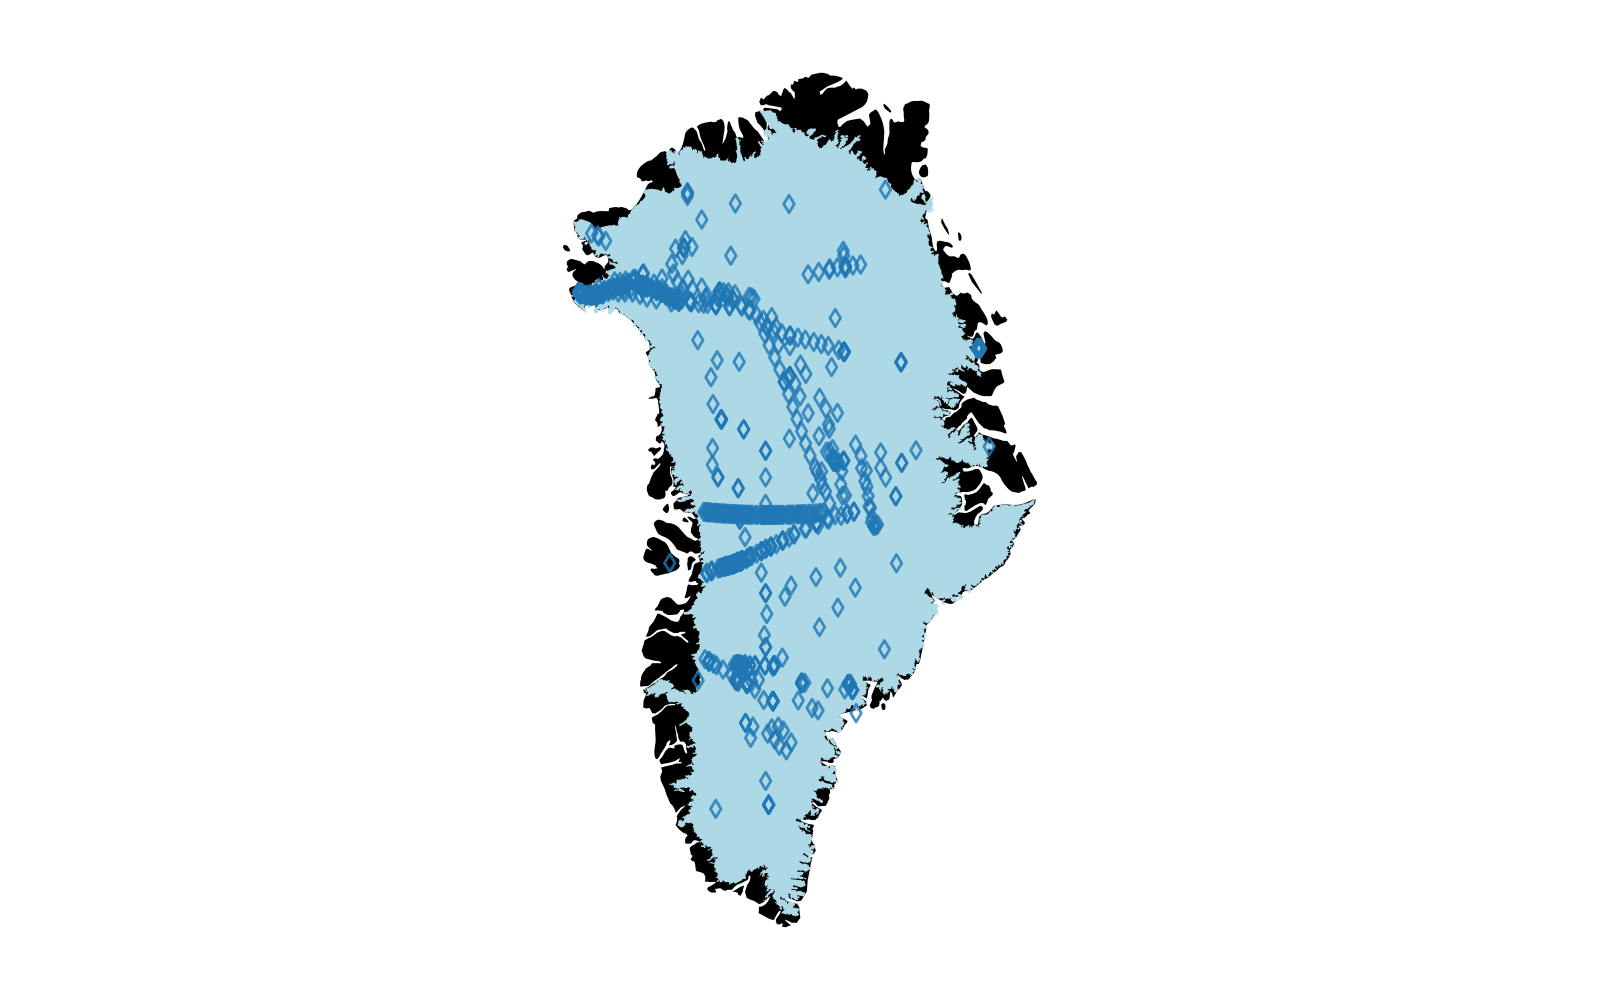
\includegraphics[width=0.45\textwidth]{figures/density_map_greenland.png}
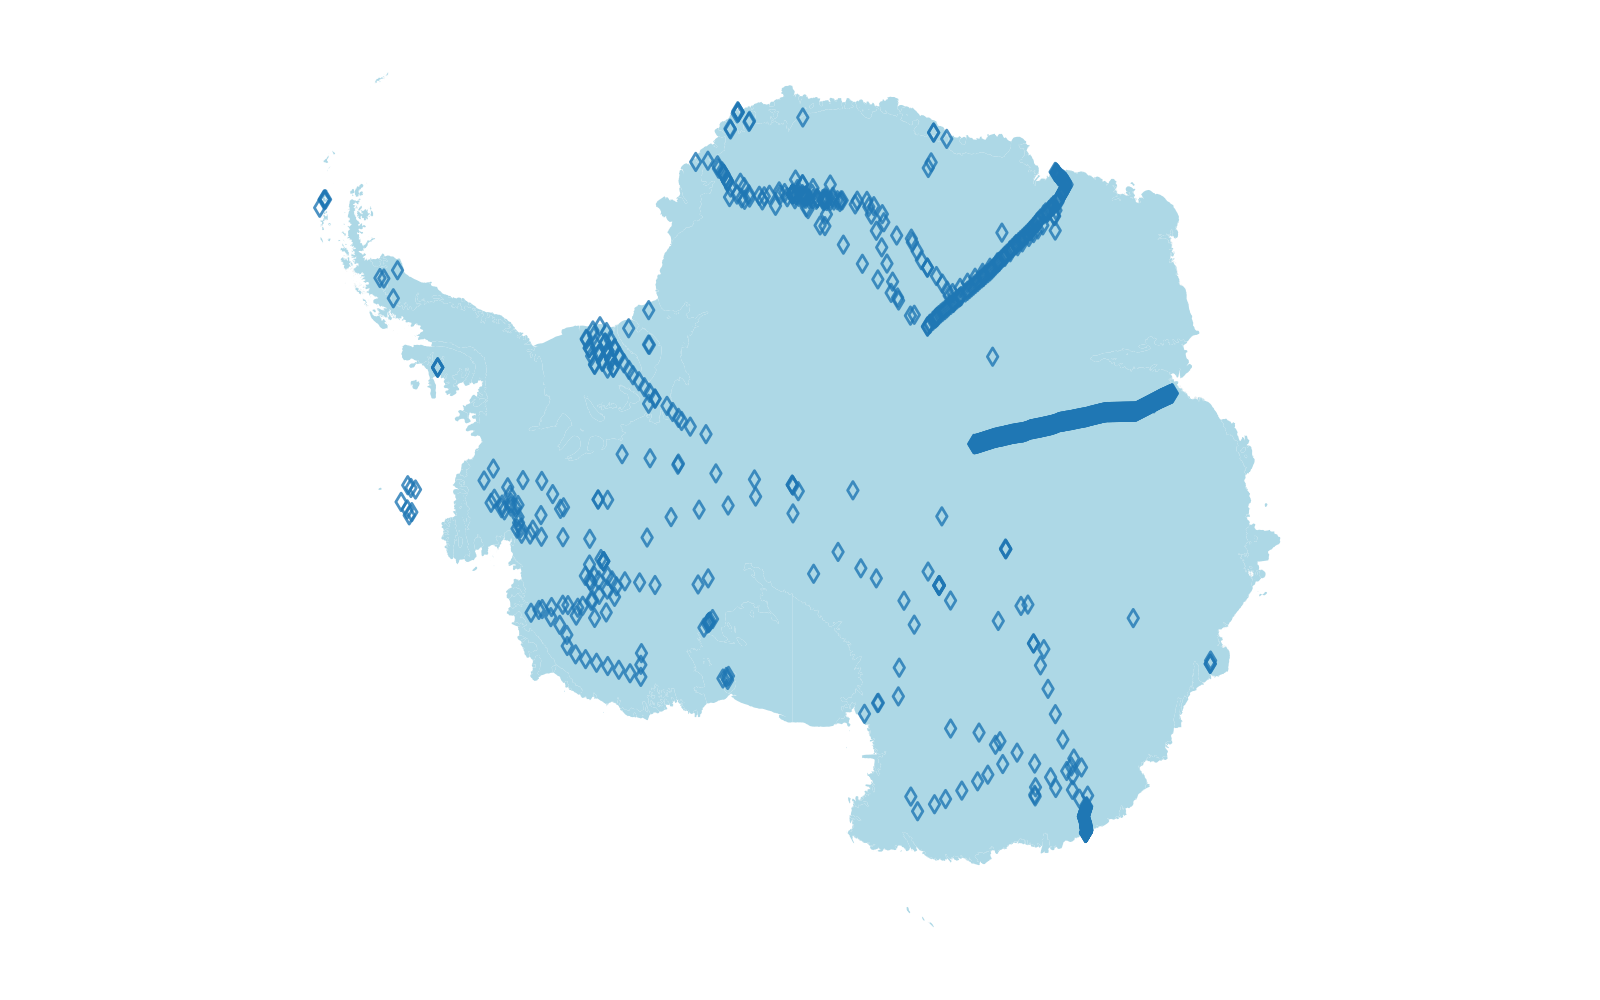
\includegraphics[width=0.45\textwidth]{figures/density_map_antarctica.png}
\end{figure}

\begin{figure}[!htb]
\caption{Composition of the density dataset in Greenland}
\centering
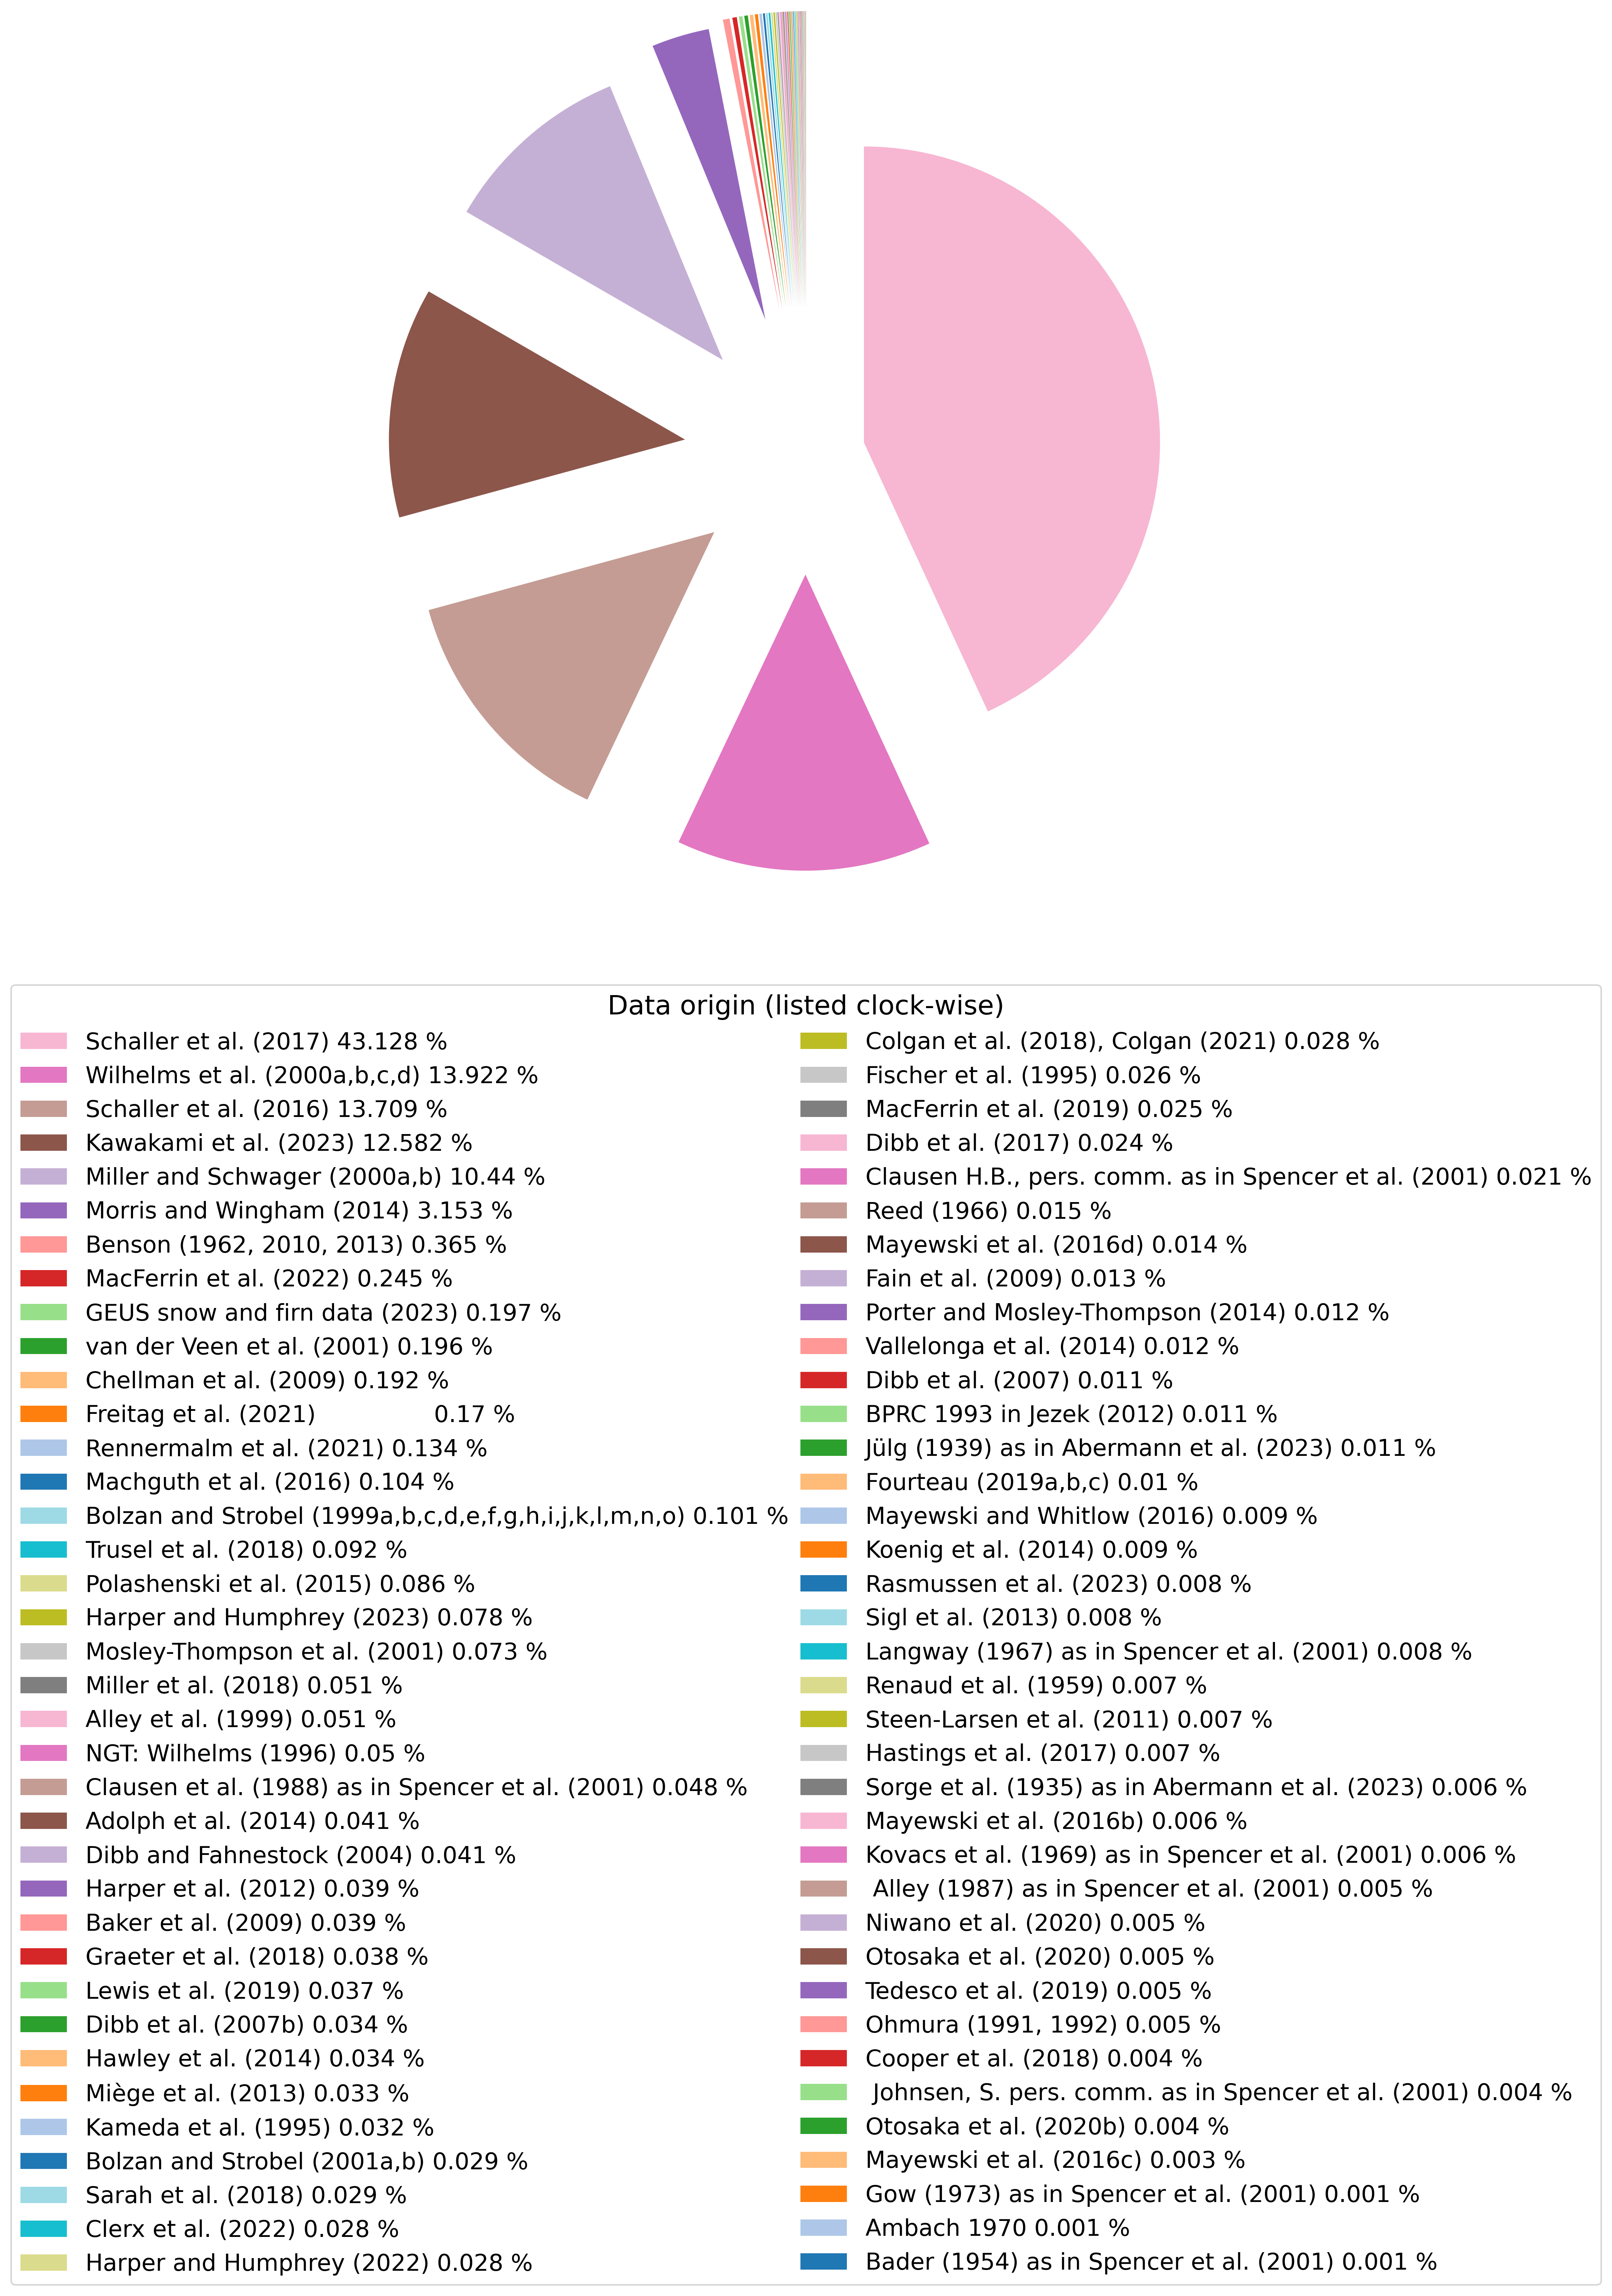
\includegraphics[scale=0.4]{figures/density_dataset_composition_greenland.png}
\end{figure}


\begin{figure}[!htb]
\caption{Composition of the density dataset in Antarctica}
\centering
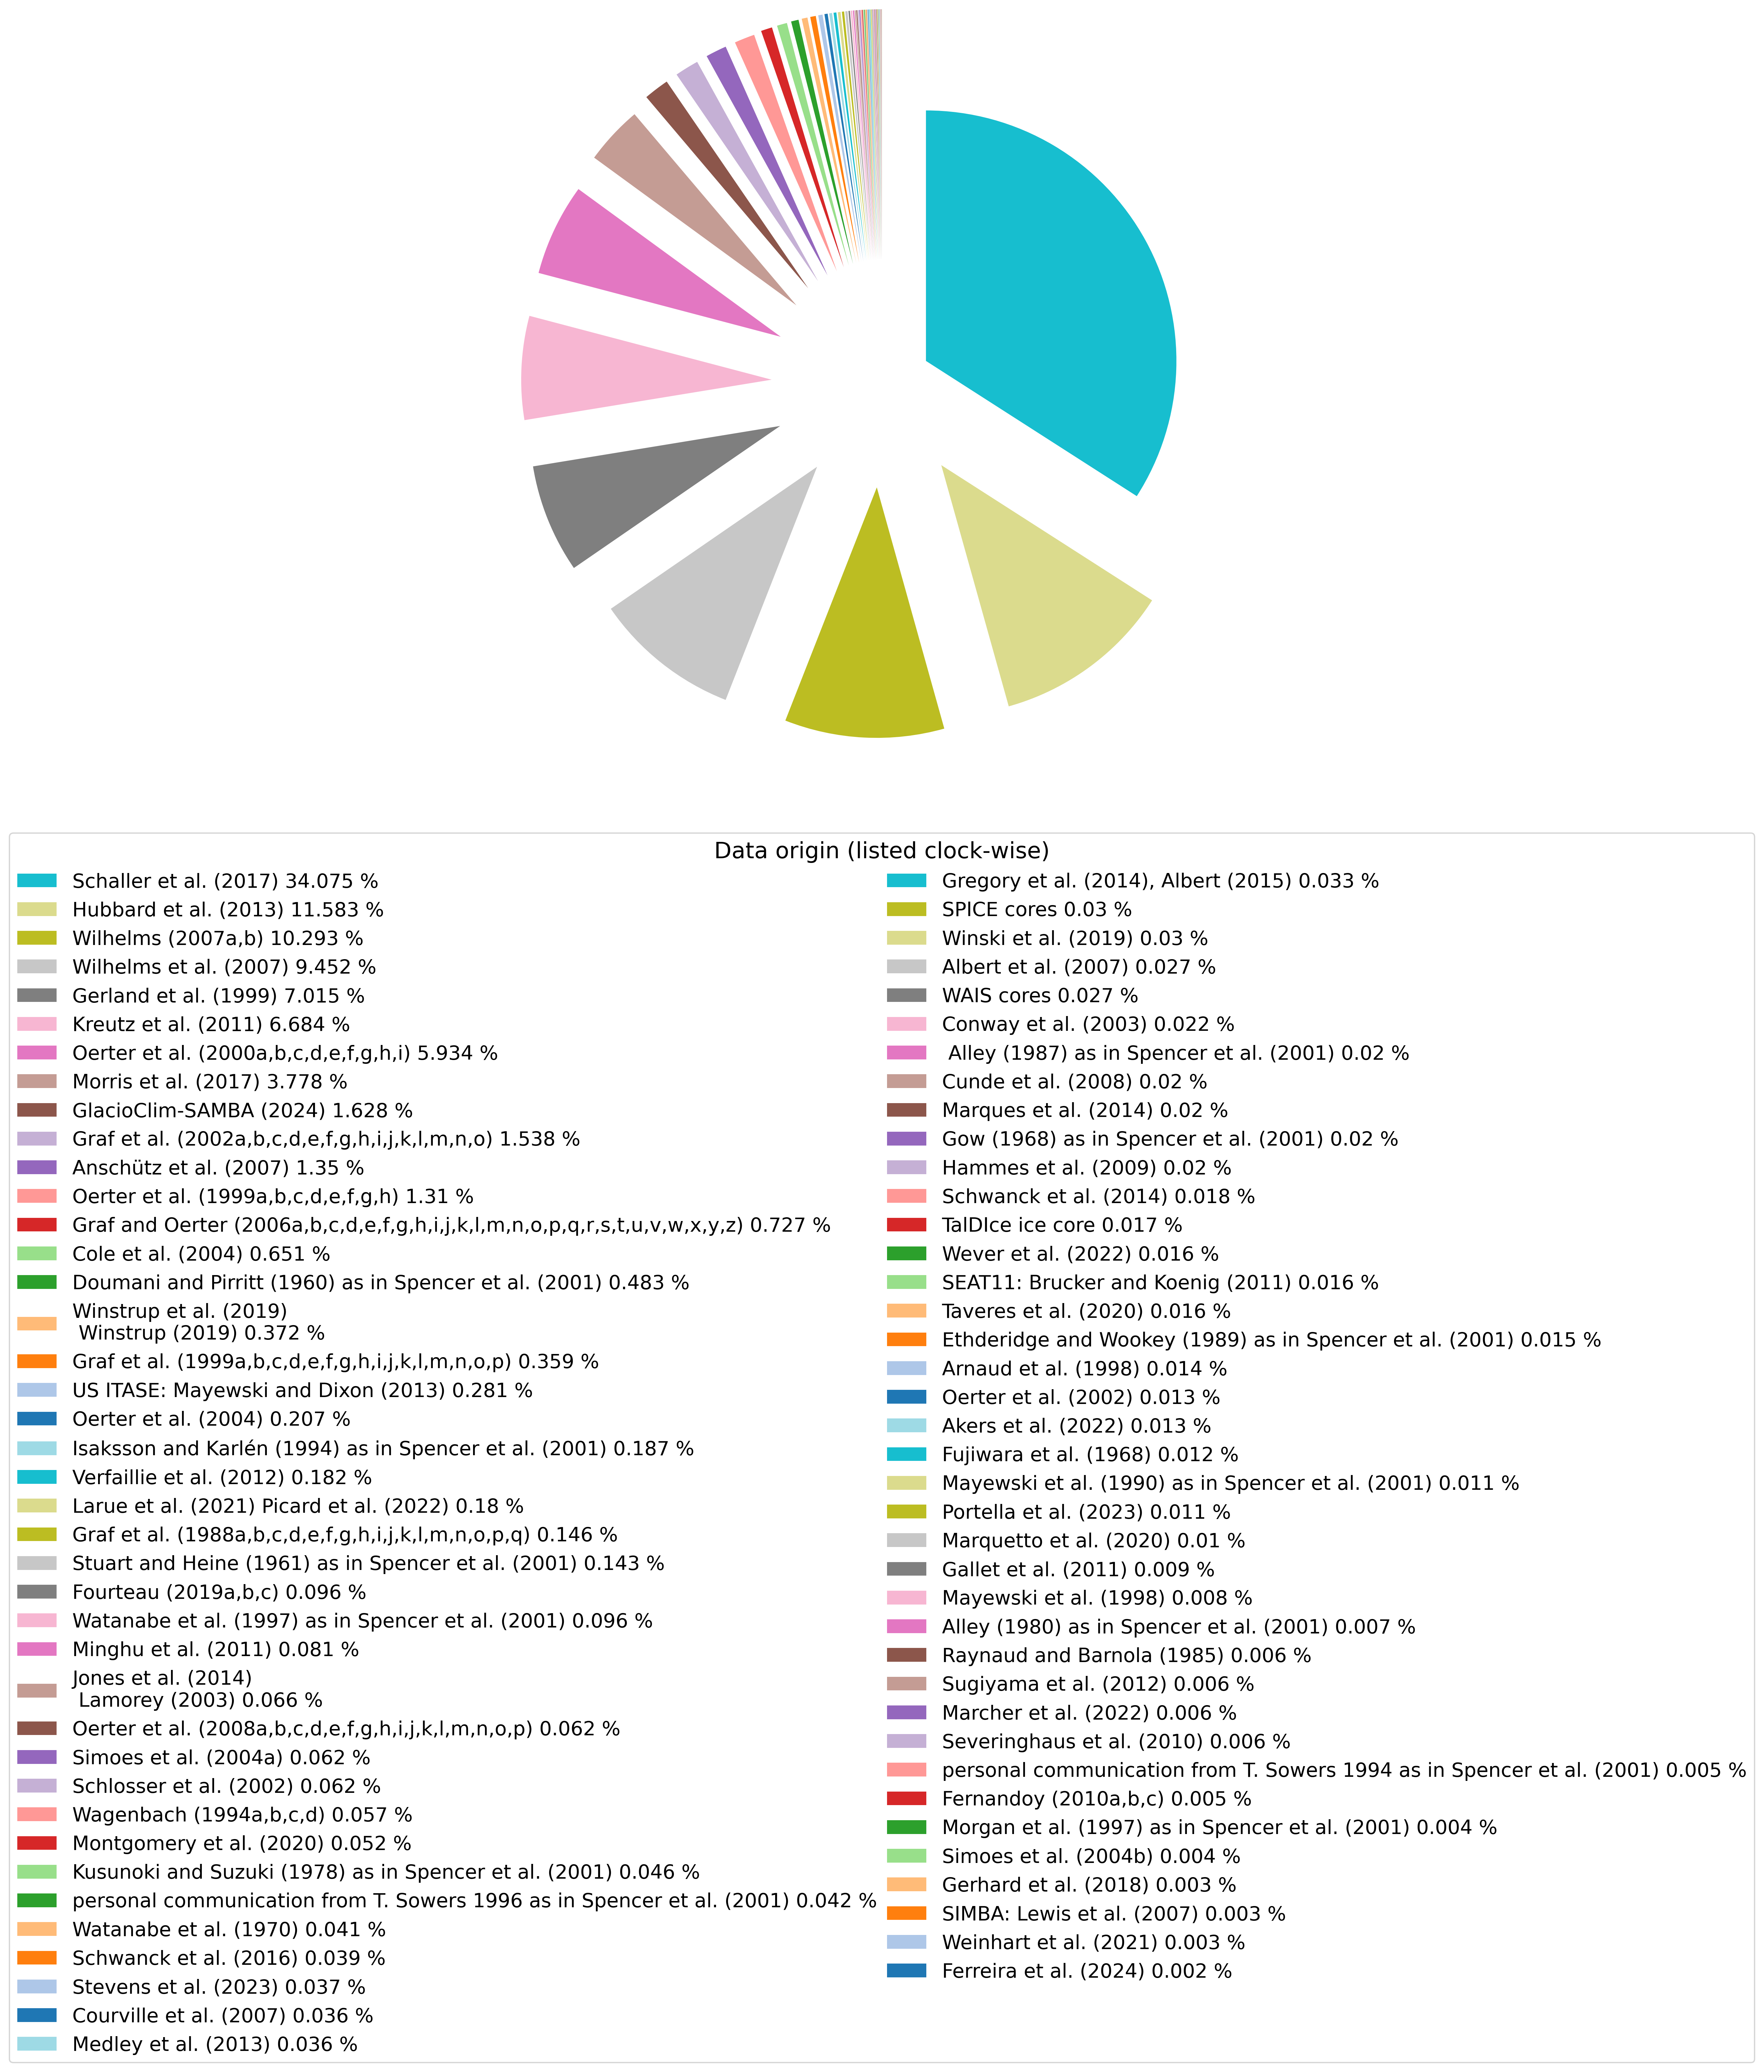
\includegraphics[scale=0.4]{figures/density_dataset_composition_antarctica.png}
\end{figure}

\FloatBarrier
\subsection{SMB}
\small
\csvautolongtable[
 table head=\caption{Origins and temporal coverage of the SMB data in Greenland}\label{tab:comp_smb_gr}\\\hline
               \csvlinetotablerow\\\hline
               \endfirsthead\hline
               \csvlinetotablerow\\\hline
               \endhead\hline
               \endfoot,
               respect all]{tables/composition_SMB_greenland.csv}
\small
\csvautolongtable[
 table head=\caption{Origins and temporal coverage of the SMB data in Antarctica}\label{tab:comp_smb_ant}\\\hline
               \csvlinetotablerow\\\hline
               \endfirsthead\hline
               \csvlinetotablerow\\\hline
               \endhead\hline
               \endfoot,
               respect all]{tables/composition_SMB_antarctica.csv}

\begin{figure}[!htb]
\caption{Spatial distribution of the SMB measurements in Greenland (left) and Antarctica (right)}
\centering
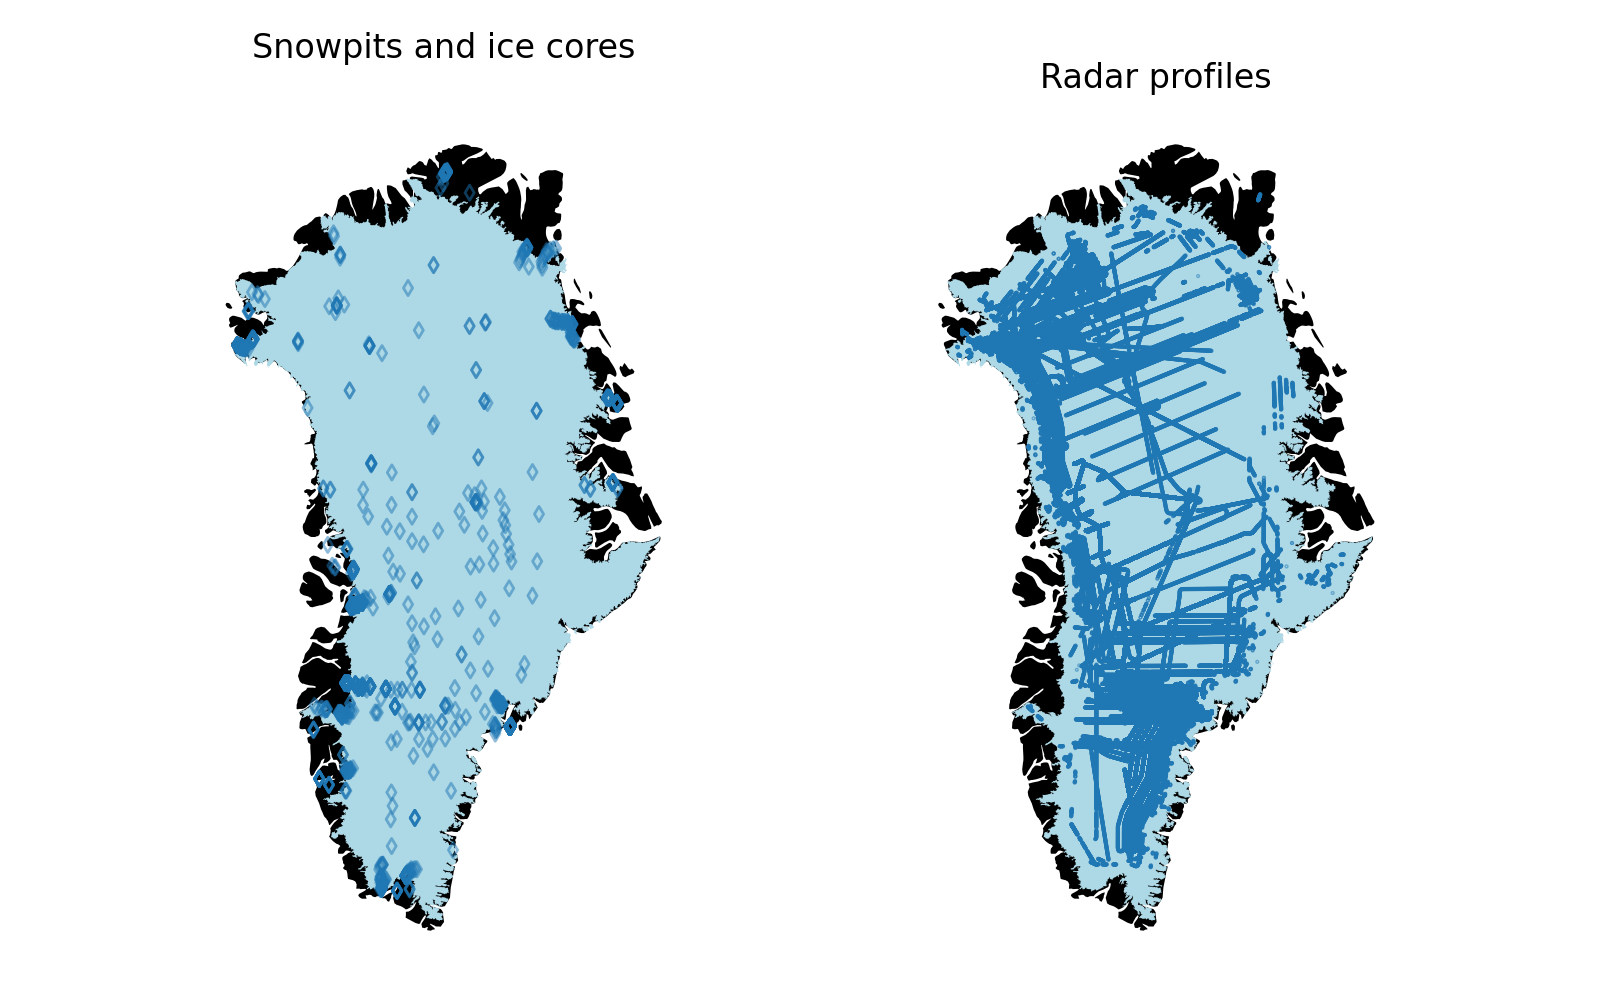
\includegraphics[width=0.45\textwidth]{figures/SMB_map_greenland.png}
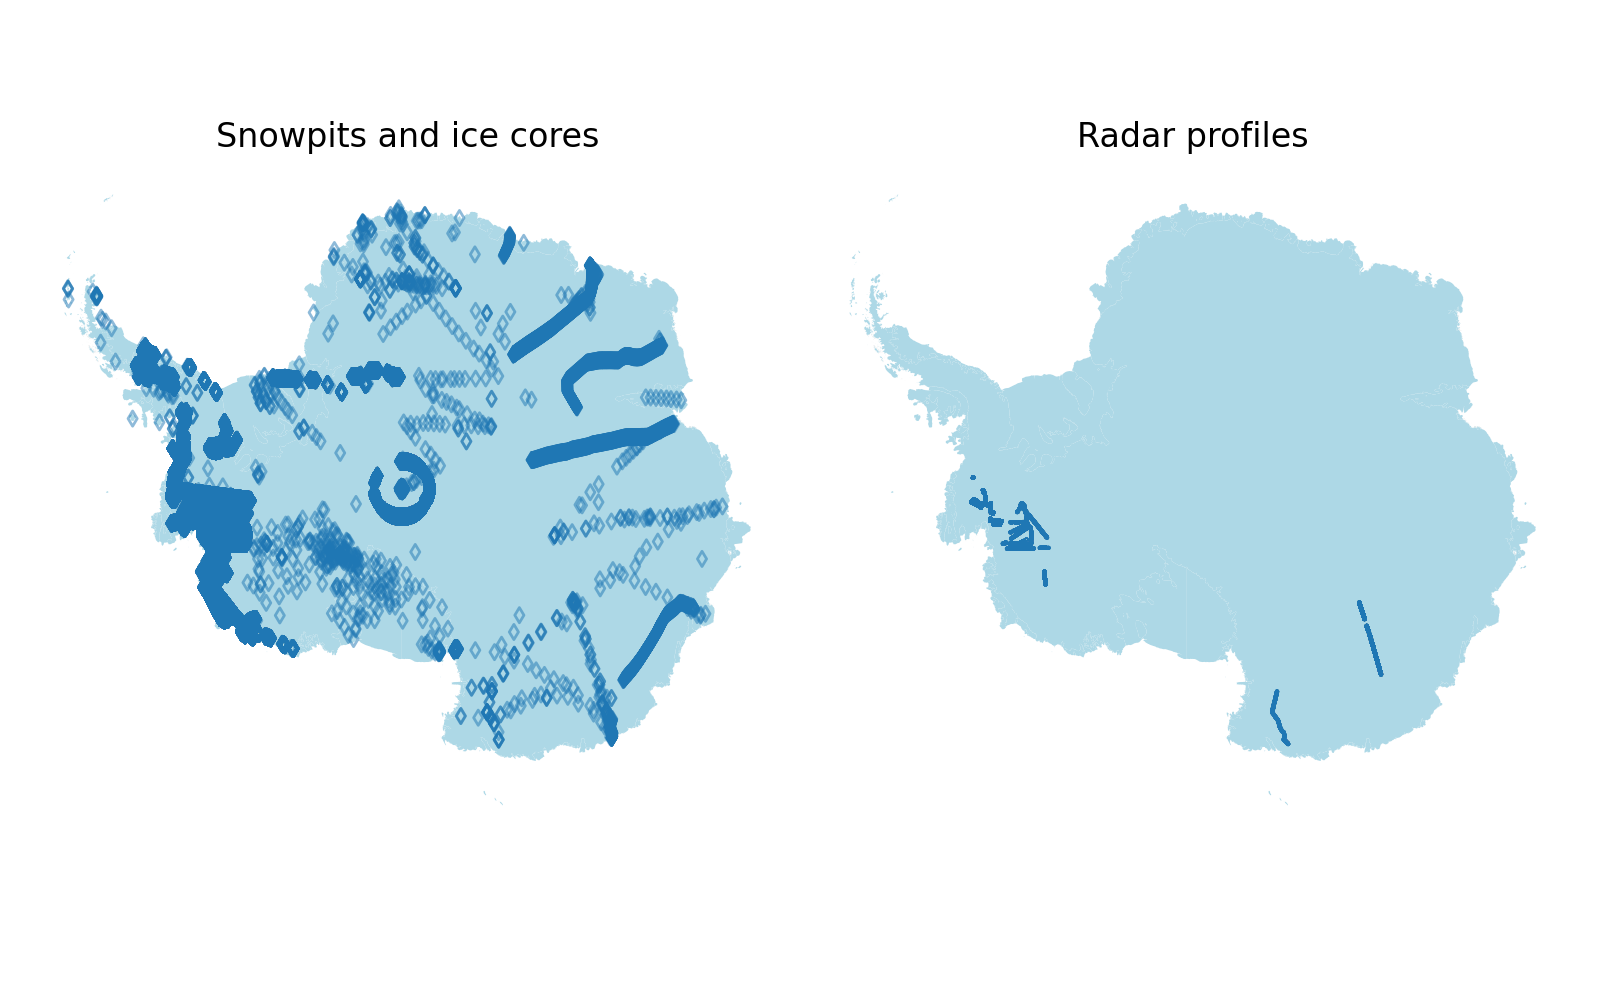
\includegraphics[width=0.45\textwidth]{figures/SMB_map_antarctica.png}
\end{figure}

\begin{figure}[!htb]
\caption{Composition of the SMB dataset in Greenland}
\centering
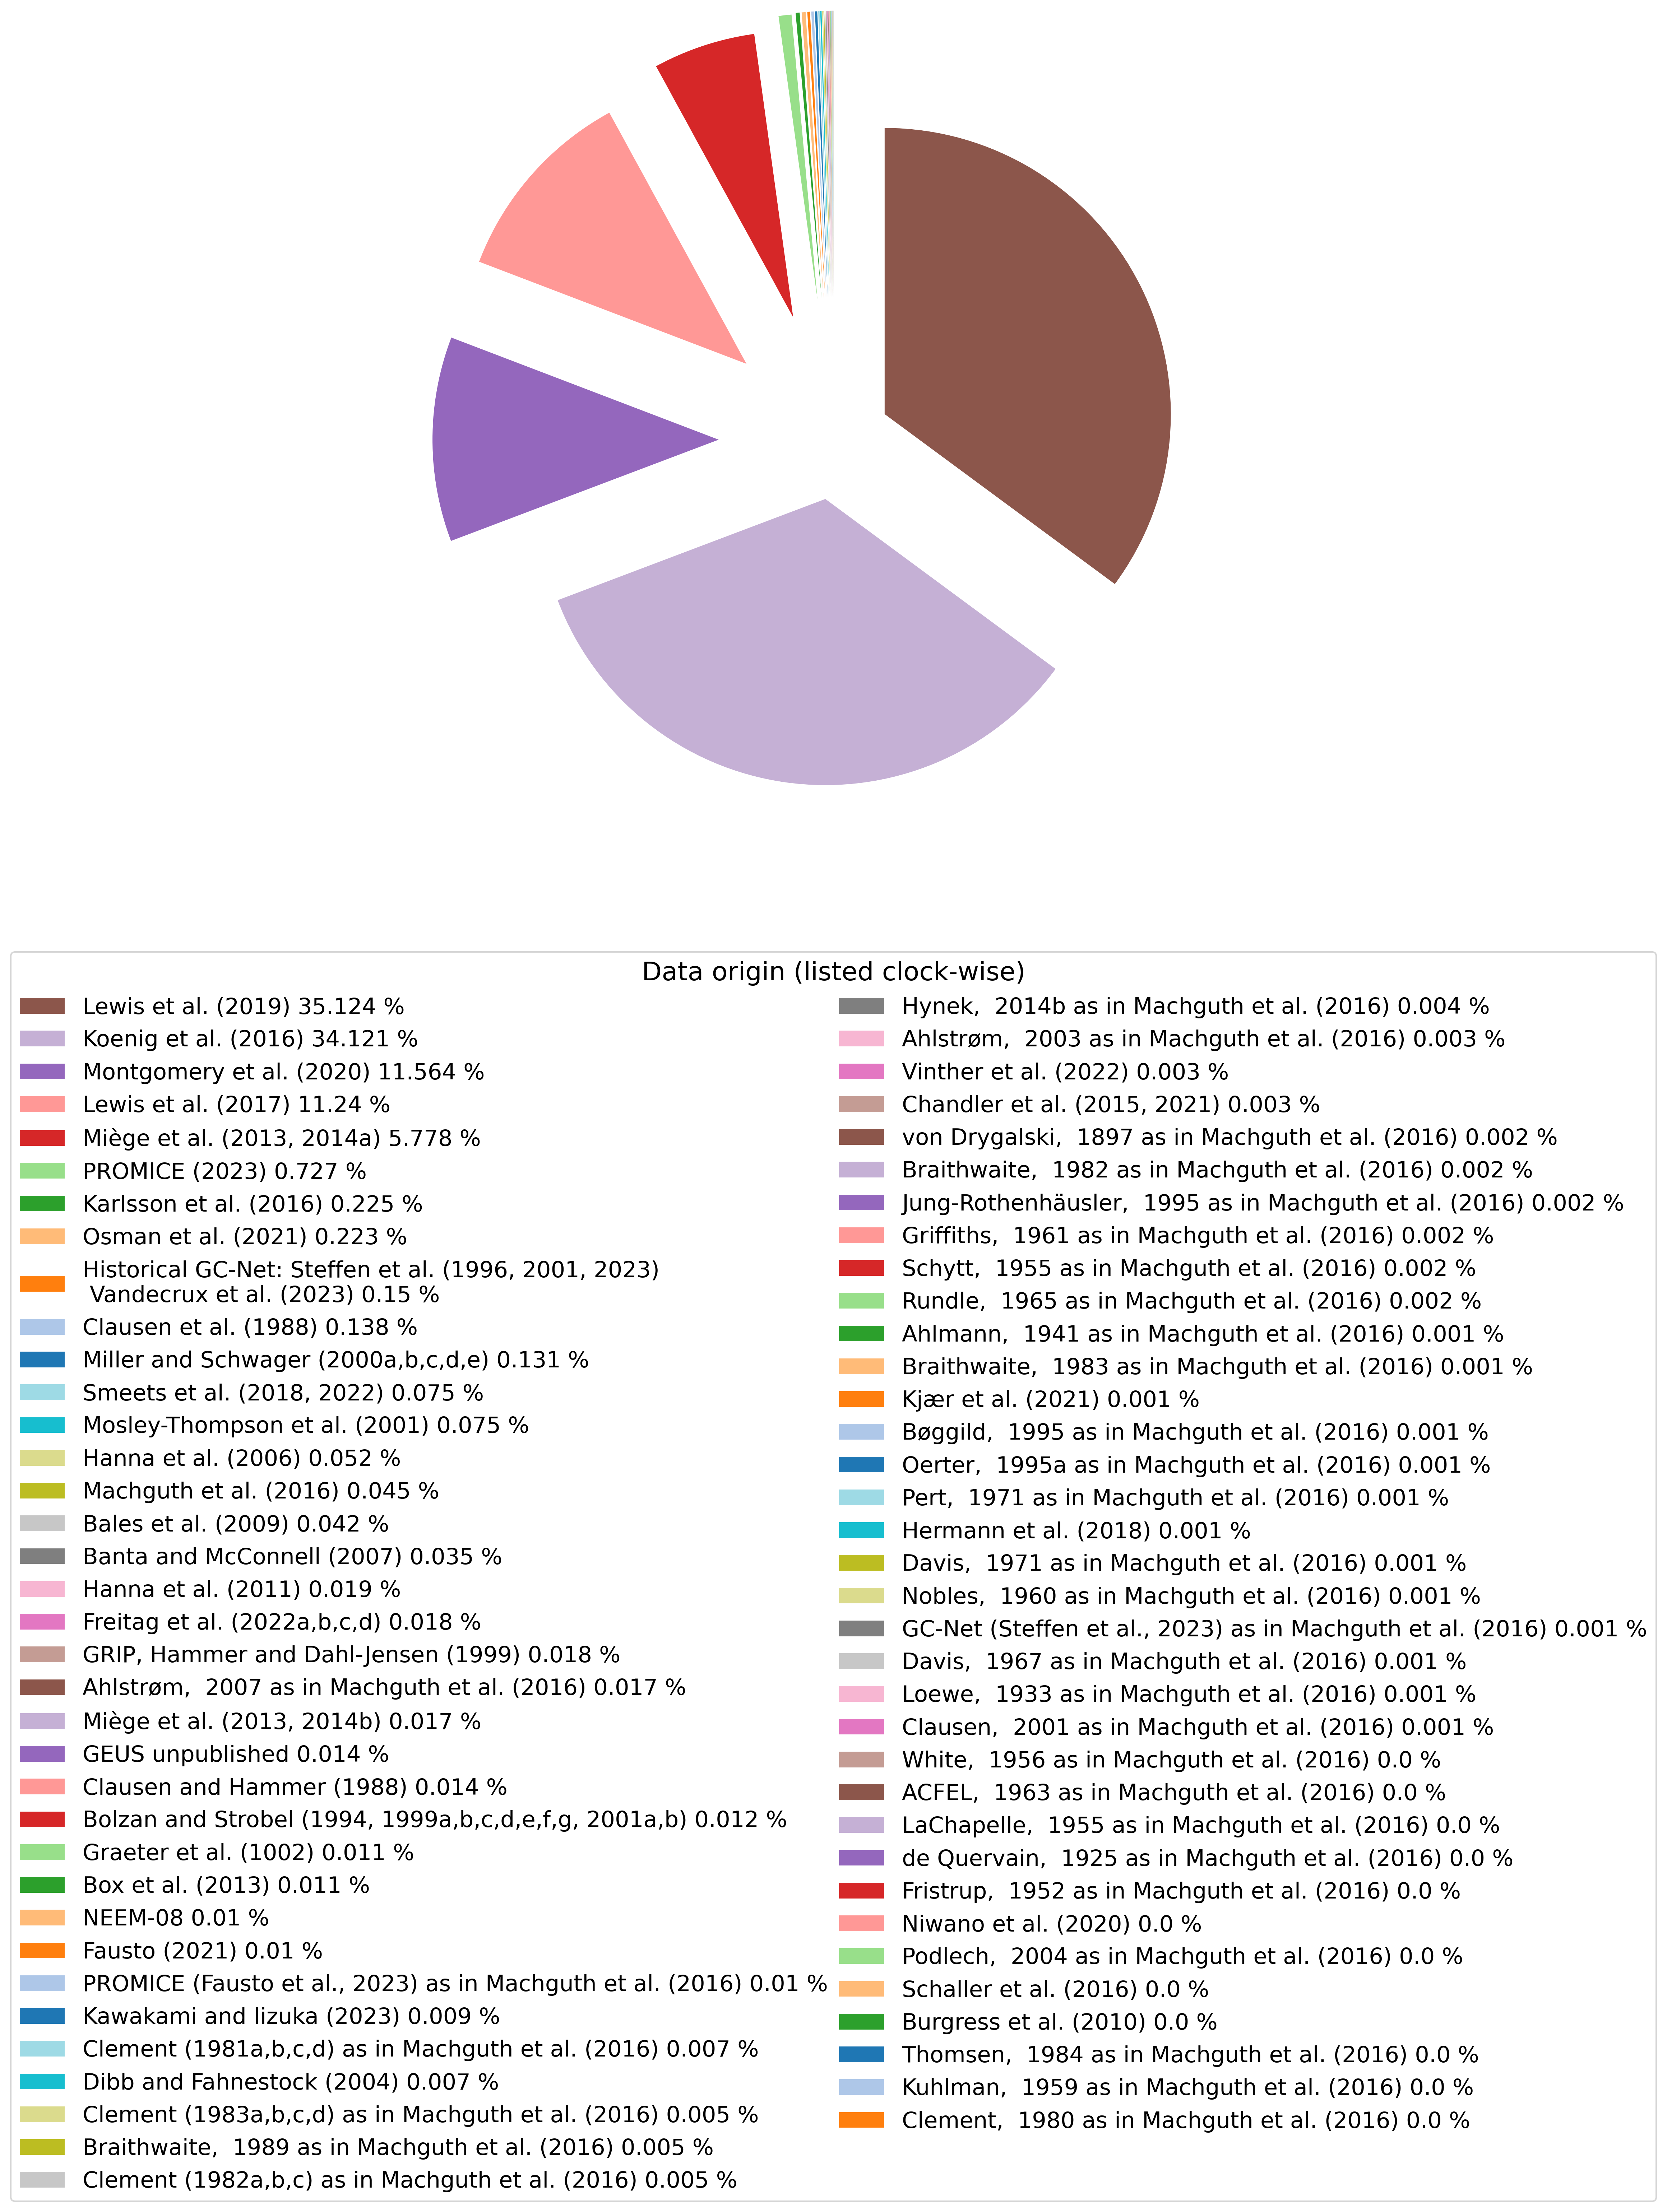
\includegraphics[scale=0.4]{figures/SMB_dataset_composition_greenland.png}
\end{figure}


\begin{figure}[!htb]
\caption{Composition of the SMB dataset in Antarctica}
\centering
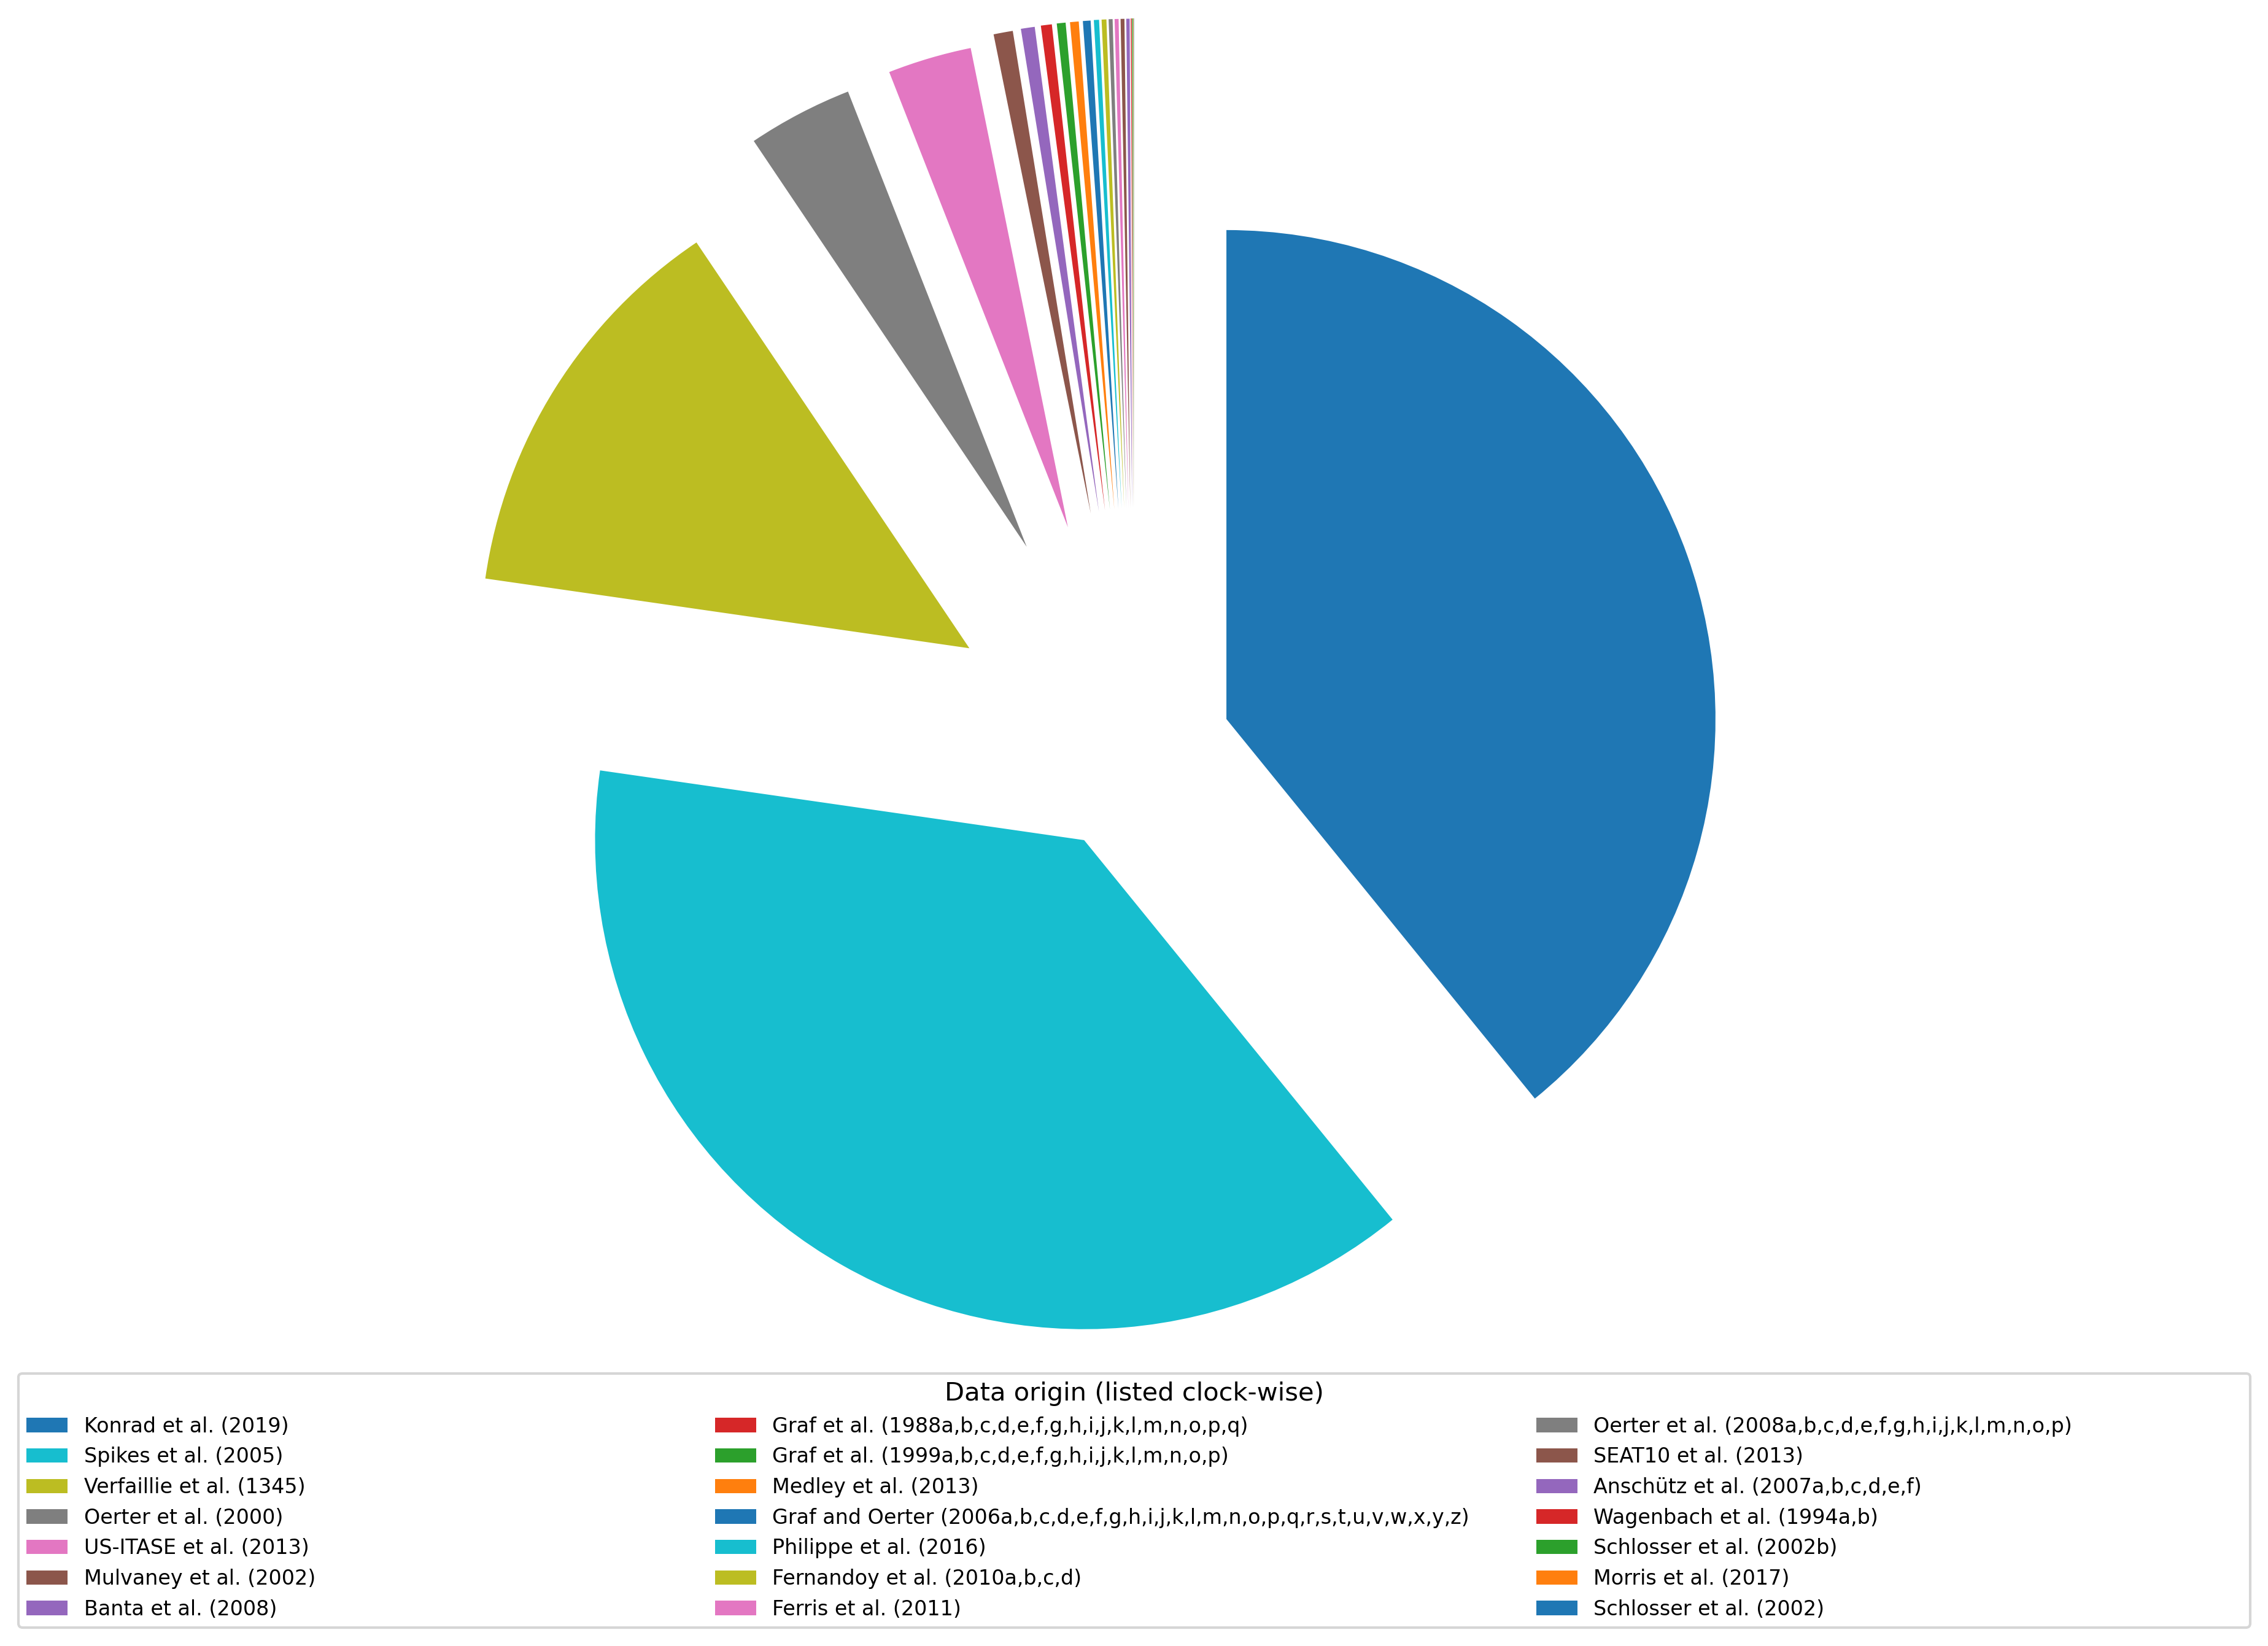
\includegraphics[scale=0.4]{figures/SMB_dataset_composition_antarctica.png}
\end{figure}

\FloatBarrier
\subsection{Temperature}
\small
\csvautolongtable[
 table head=\caption{Origins and temporal coverage of the temperature data in Greenland}\label{tab:comp_temp_gr}\\\hline
               \csvlinetotablerow\\\hline
               \endfirsthead\hline
               \csvlinetotablerow\\\hline
               \endhead\hline
               \endfoot,
               respect all]{tables/composition_temperature_greenland.csv}
\small
\csvautolongtable[
 table head=\caption{Origins and temporal coverage of the temperature data in Antarctica}\label{tab:comp_temp_ant}\\\hline
               \csvlinetotablerow\\\hline
               \endfirsthead\hline
               \csvlinetotablerow\\\hline
               \endhead\hline
               \endfoot,
               respect all]{tables/composition_temperature_antarctica.csv}

\begin{figure}[!htb]
\caption{Spatial distribution of the temperature measurements in Greenland (left) and Antarctica (right)}
\centering
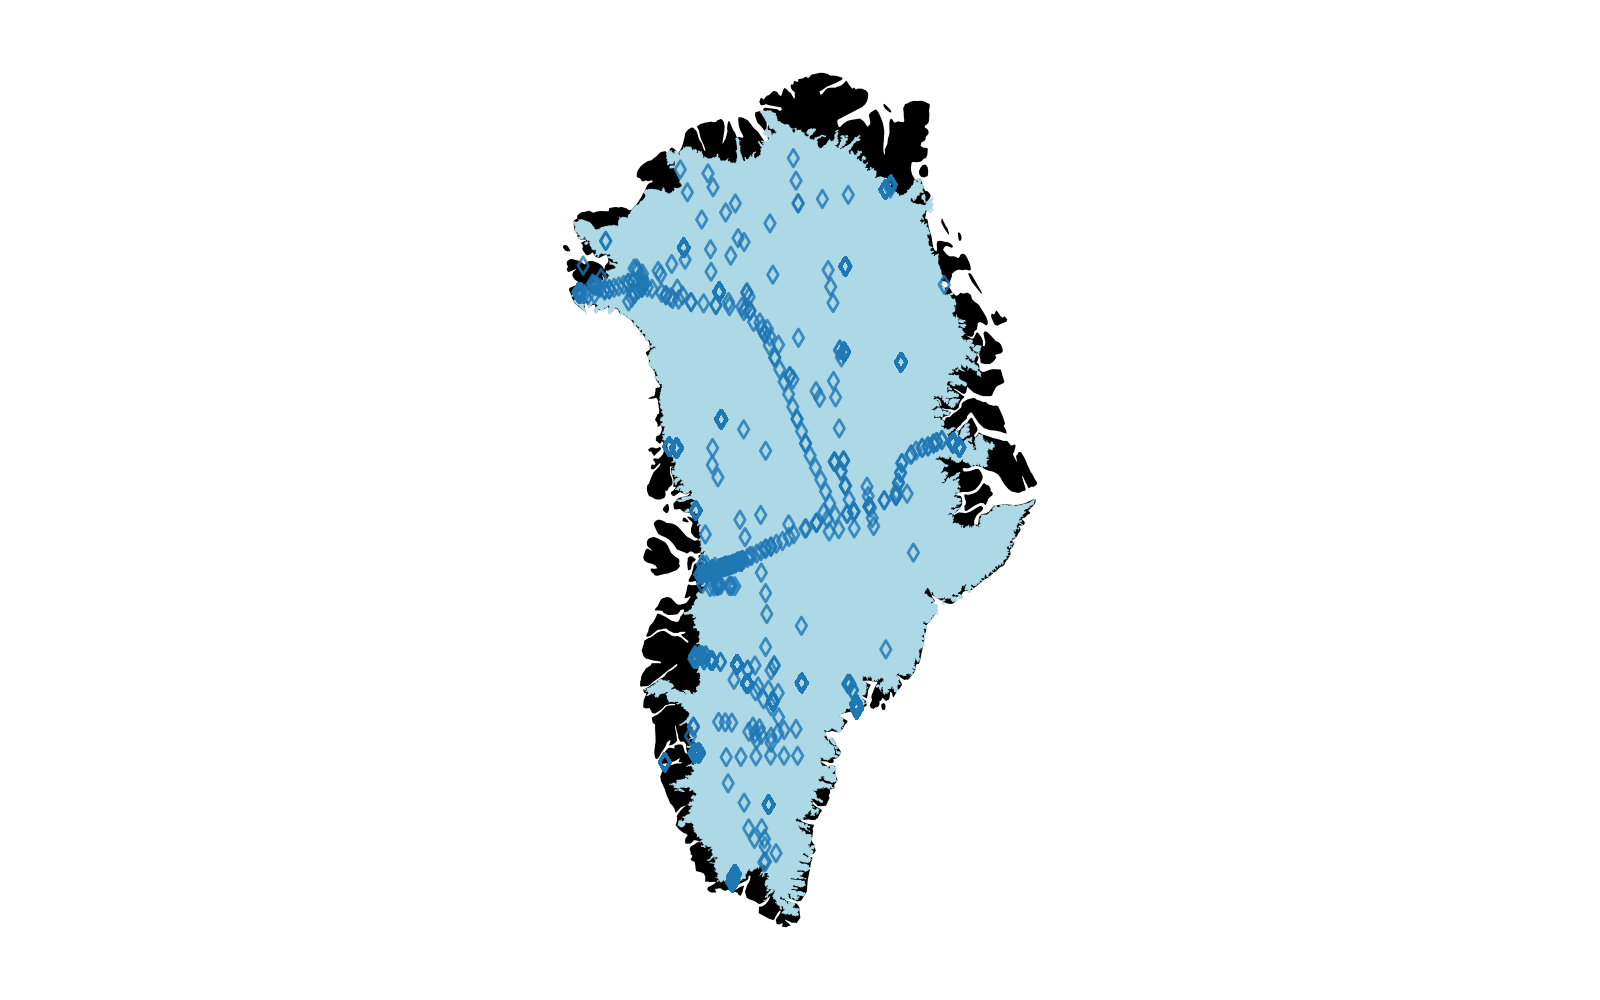
\includegraphics[width=0.45\textwidth]{figures/temperature_map_greenland.png}
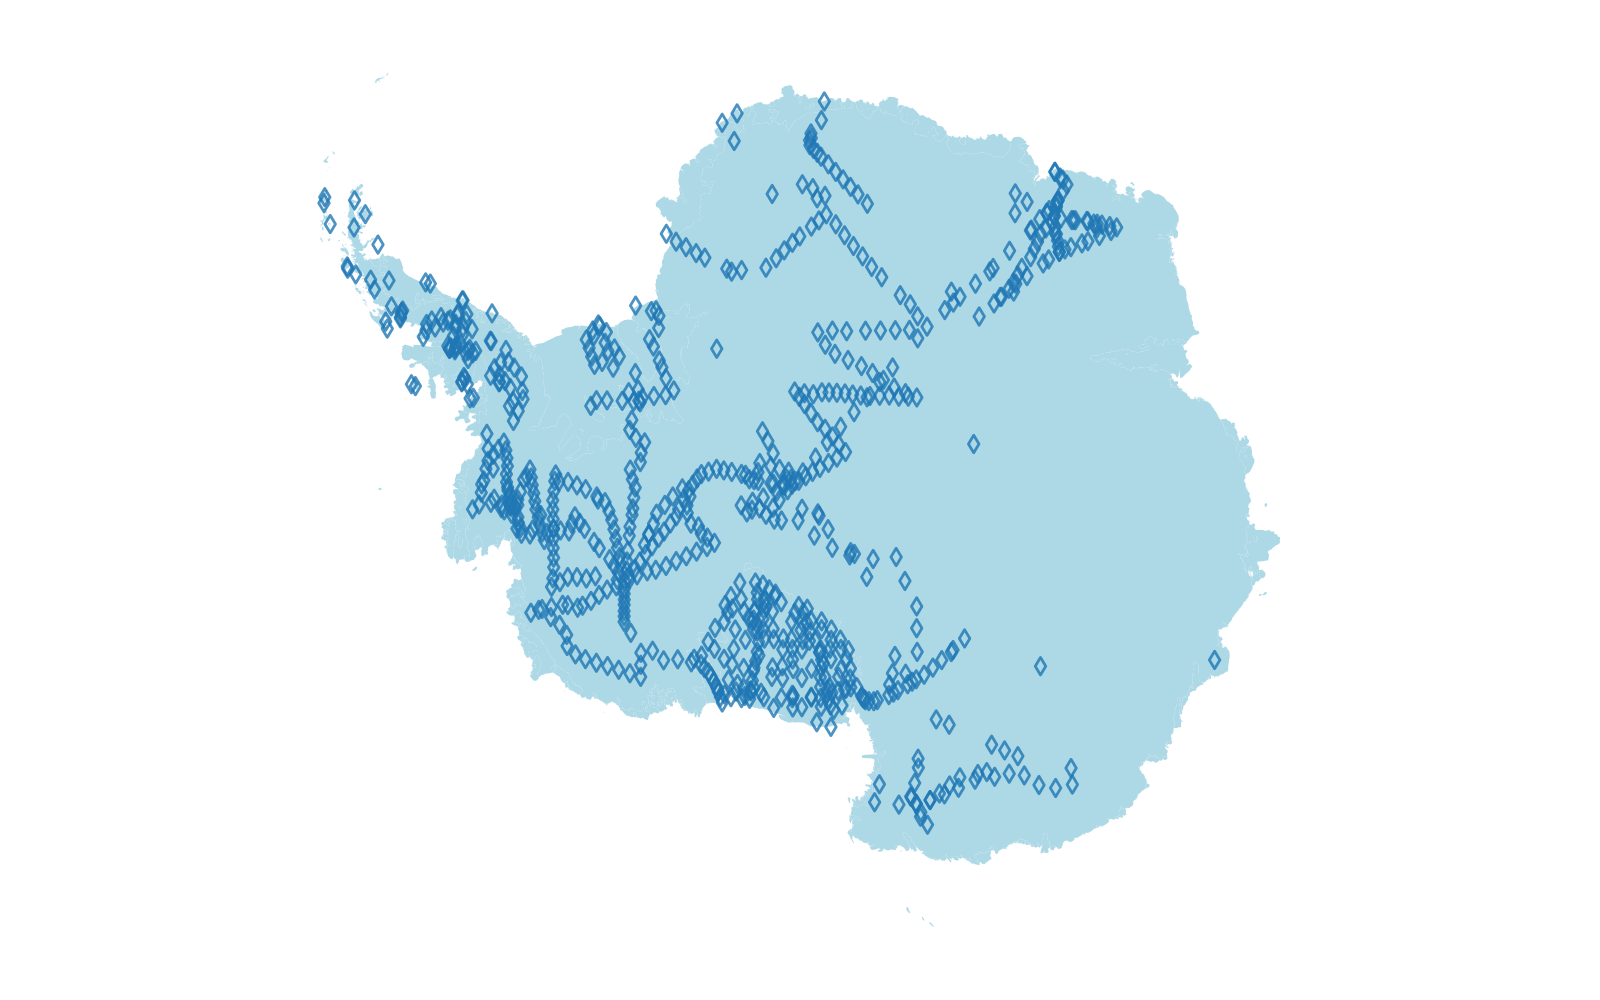
\includegraphics[width=0.45\textwidth]{figures/temperature_map_antarctica.png}
\end{figure}

\begin{figure}[!htb]
\caption{Composition of the temperature dataset in Greenland}
\centering
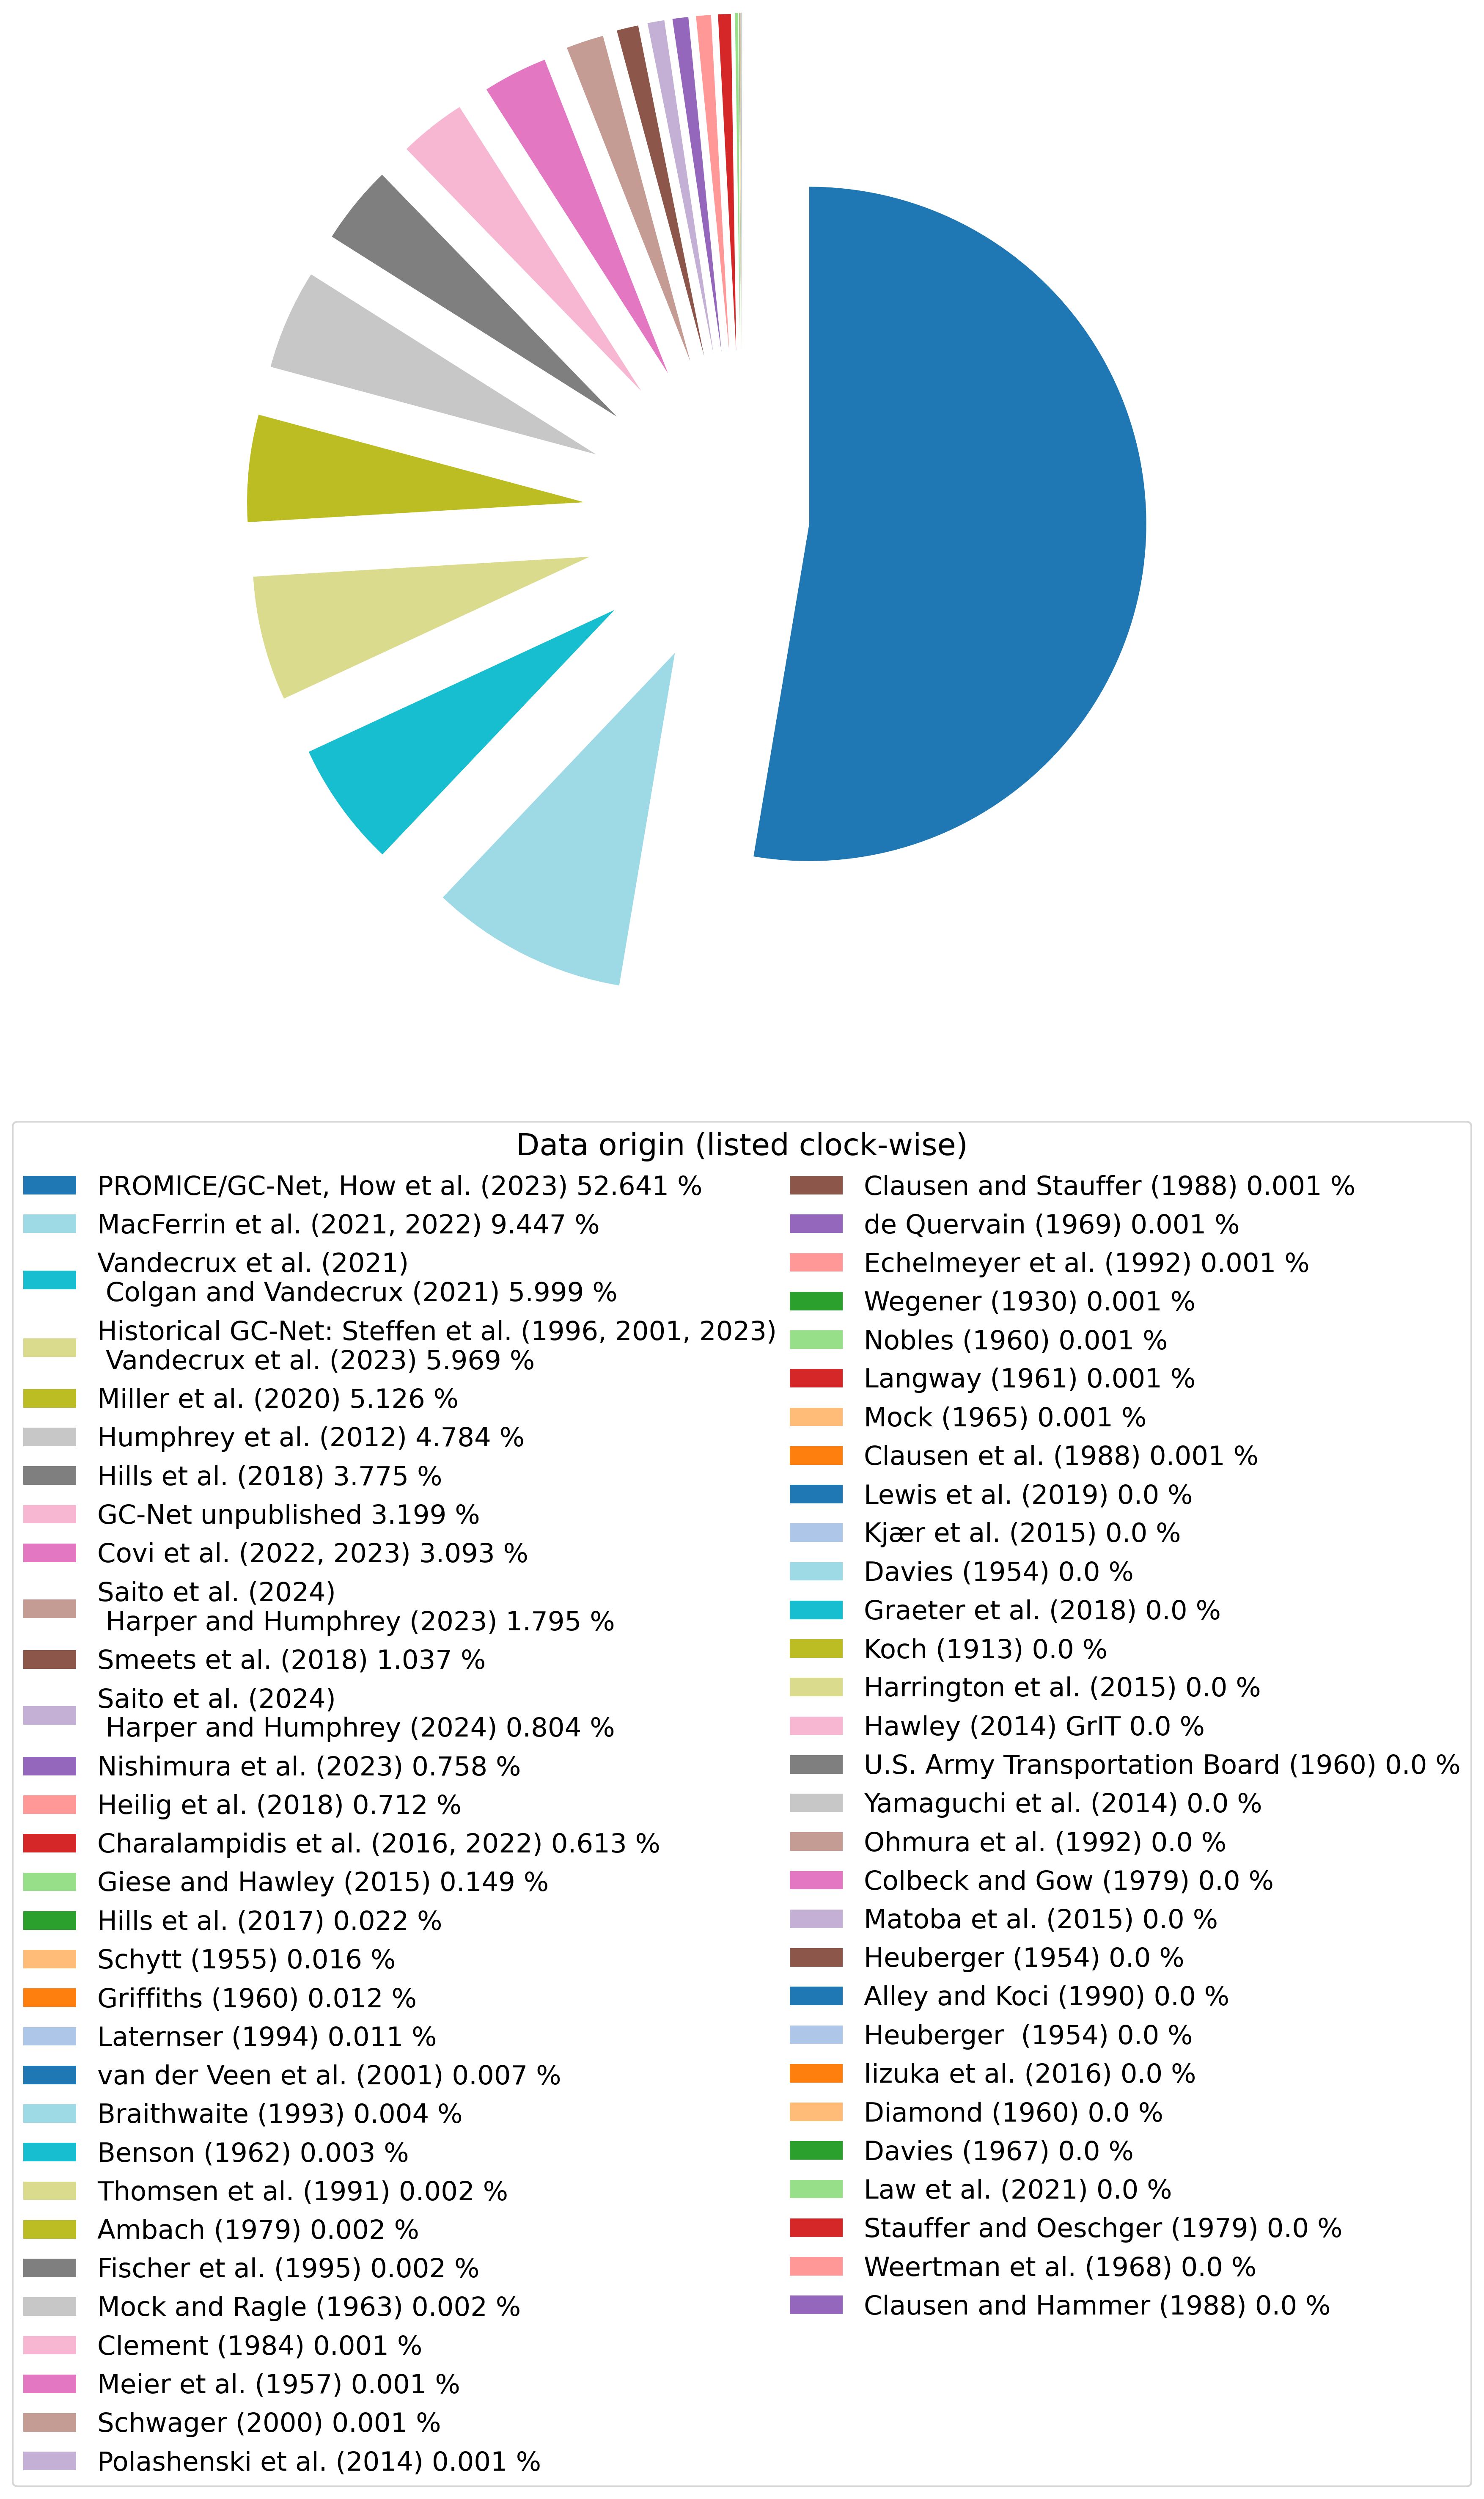
\includegraphics[scale=0.4]{figures/temperature_dataset_composition_greenland.png}
\end{figure}


\begin{figure}[!htb]
\caption{Composition of the temperature dataset in Antarctica}
\centering
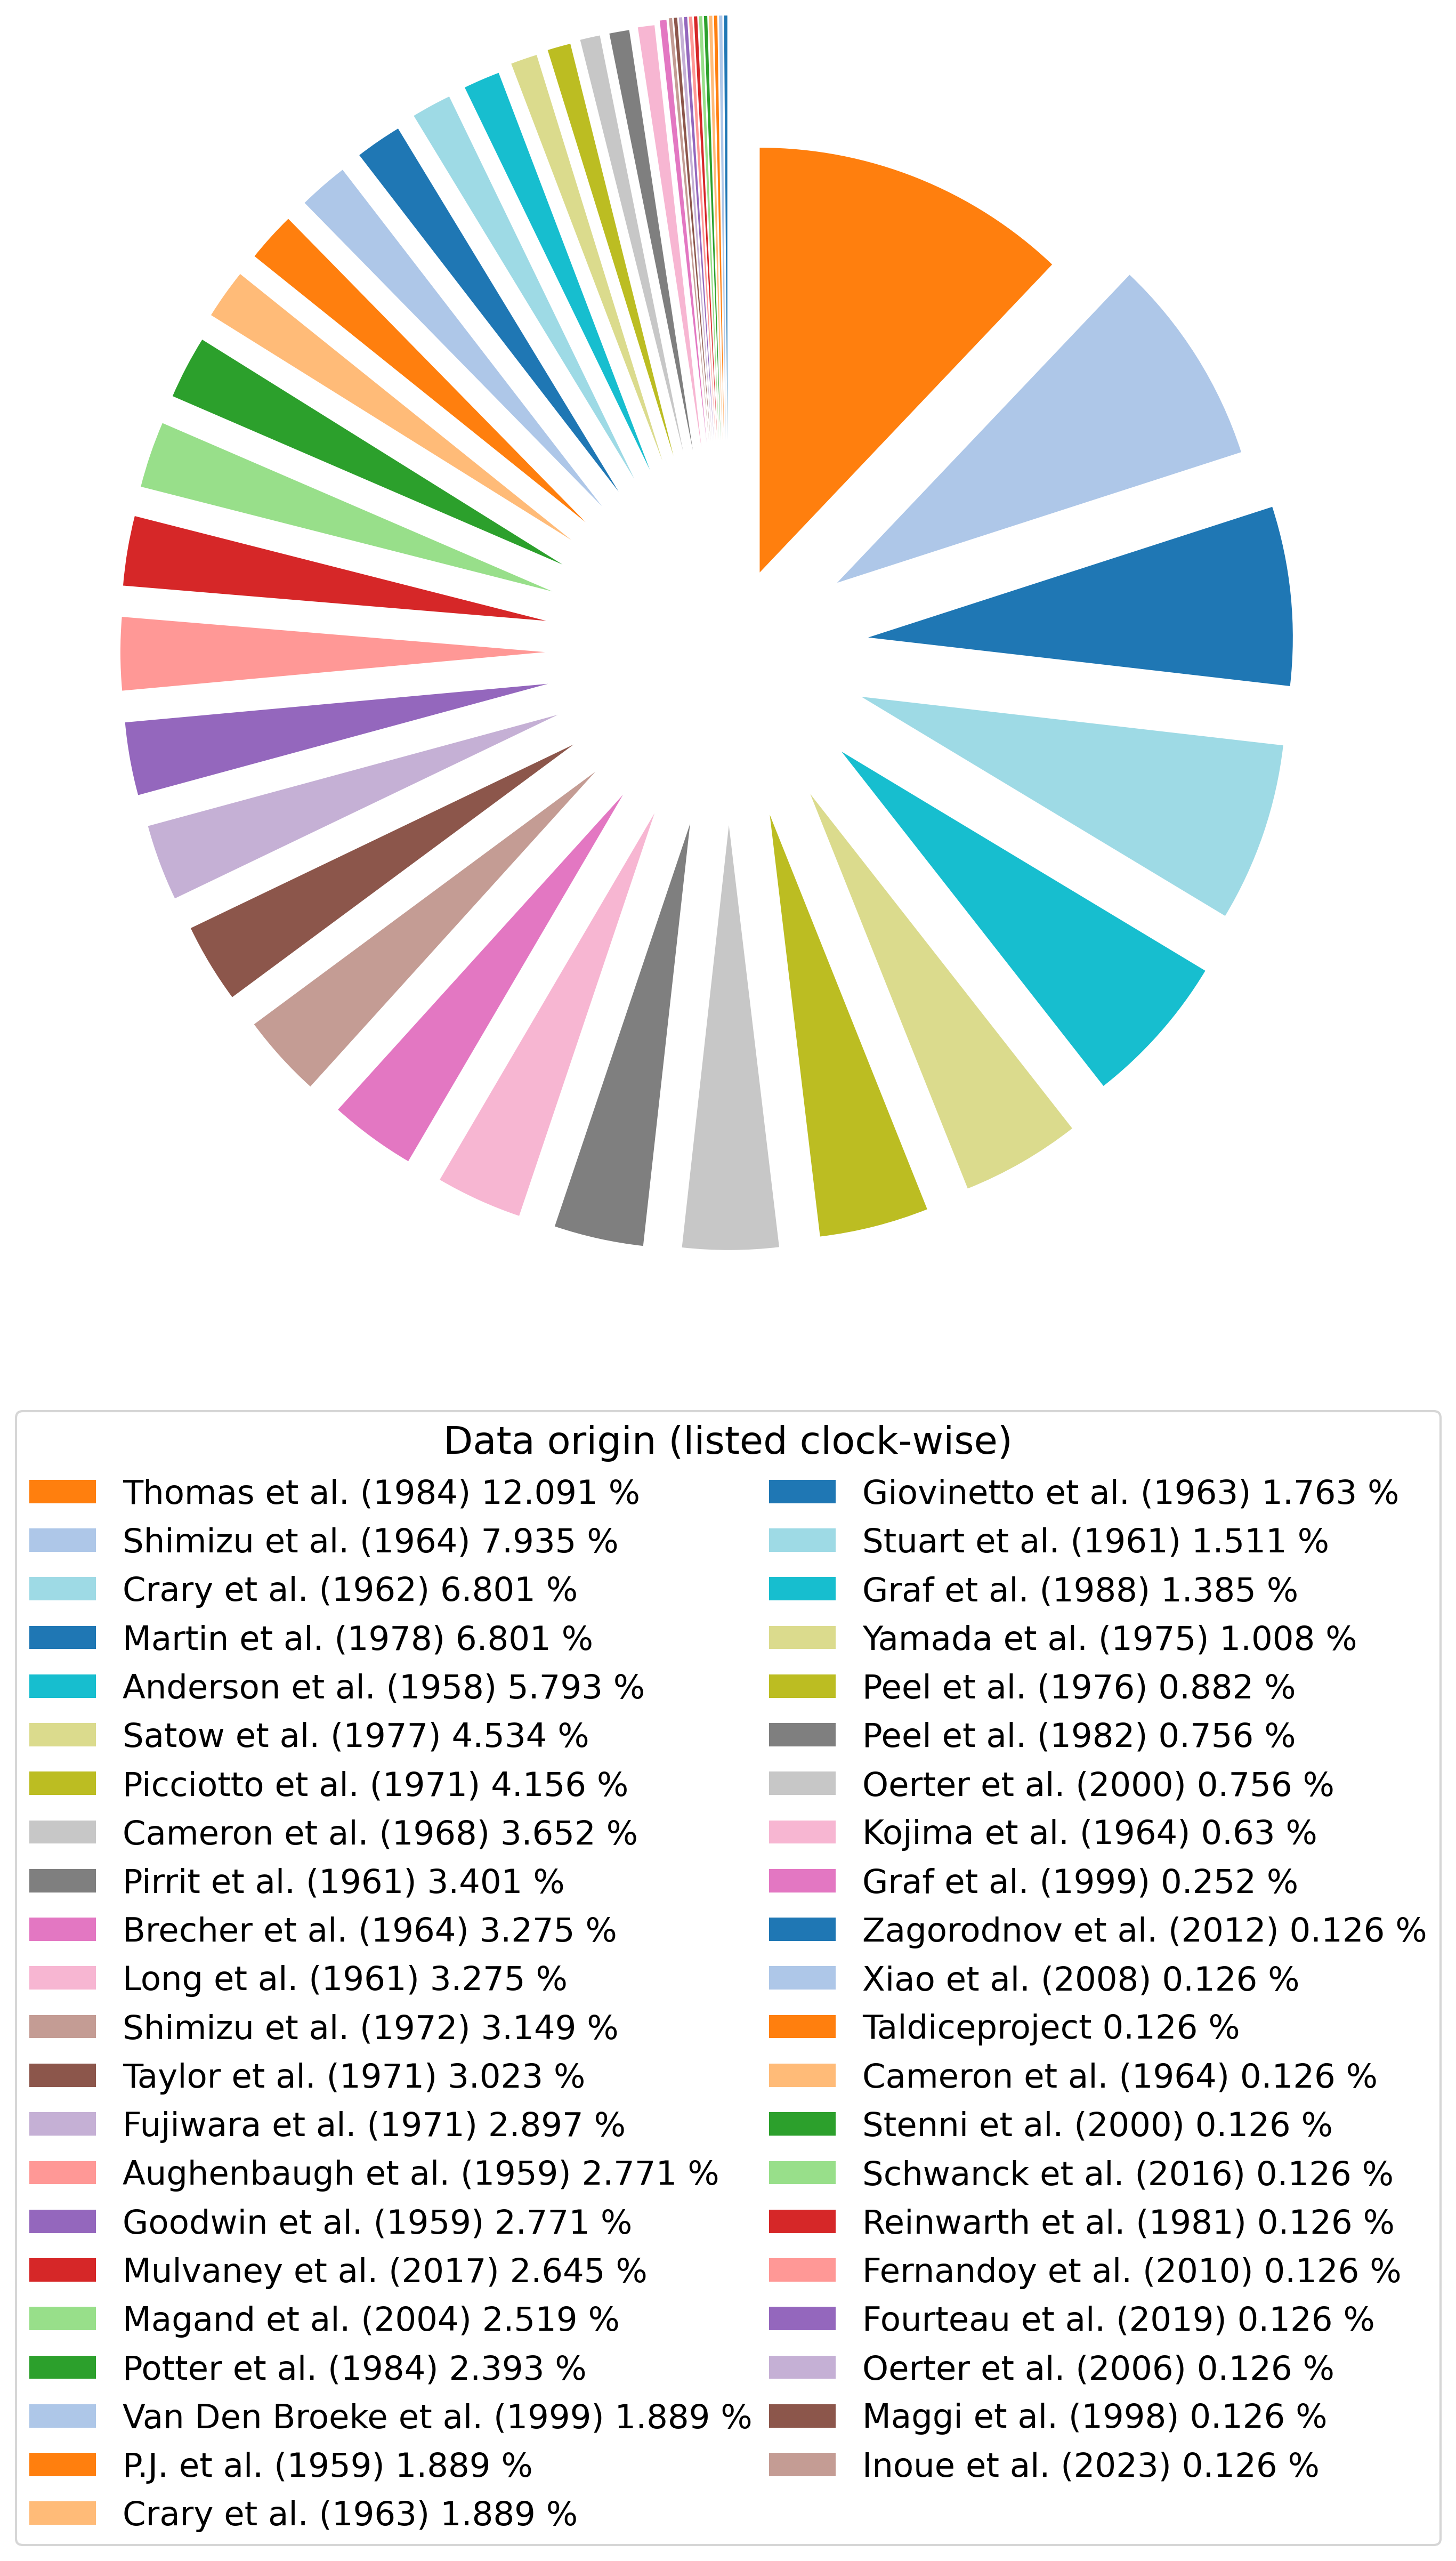
\includegraphics[scale=0.4]{figures/temperature_dataset_composition_antarctica.png}
\end{figure}

\FloatBarrier
\section{References}
\input{tables/SUMup_2024_all_references.tsv}

%\conclusions  %% \conclusions[modified heading if necessary]
%\dataavailability{TEXT} %% use this section when having only data sets available
%\codedataavailability{TEXT} 
%\noappendix       %% use this to mark the end of the appendix section
%\authorcontribution{TEXT} 
%\begin{acknowledgements}
%TEXT
%\end{acknowledgements}
%% REFERENCES
%% The reference list is compiled as follows:
%\begin{thebibliography}{}
%\bibitem[AUTHOR(YEAR)]{LABEL1}
%REFERENCE 1
%\bibitem[AUTHOR(YEAR)]{LABEL2}
%REFERENCE 2
%\end{thebibliography}

\end{document}
